\chapter{RESULTADOS OBTENIDOS Y POSIBLES MEJORAS}
\label{cap:resultados}

\section{RESULTADOS OBTENIDOS}
\subsection{Métricas de calidad de rutas}
\label{sec:metricas-calidad}

La calidad de la solución producida por el motor de optimización se evalúa sobre la instancia de
referencia congelada descrita en la Sección~\ref{sec:legacy} y en la Sección~\ref{sec:estado-actual}
(ambas fuentes, \texttt{legacy\_api} + \texttt{legacy\_app} con mediana de posición por código QR),
de $N = 1\,607$ árboles. La serie experimental completa mide además once instancias adicionales,
entre $n = 43$ y $n = 1\,607$, sobre la suite de instancias congeladas del
\hyperref[anx:suite-instancias]{Anexo 4}; esta sección reporta la instancia de referencia porque es
la que fija los criterios de aceptación del Capítulo~\ref{cap:solucion}. El conjunto no corresponde
a una única comuna: reúne una porción del arbolado disponible en ambas bases legadas, elegida por
reproducibilidad y no la totalidad del universo importable (Sección~\ref{sec:legacy}).
Se emplean los parámetros temporales por defecto ($T_{\min} = 7\,200$\,s y $T_{\max} = 10\,800$\,s),
un tiempo de servicio de 2 minutos por árbol y los \textit{defaults} de producción del motor: la
estrategia \texttt{spatial\_term} ---que agrega al objetivo un término de dispersión geográfica,
véase la Sección~\ref{sec:estrategias}--- y un tiempo límite de \textit{solver} de 120\,s, que es el
valor que produce la heurística $\min(30 + 1{,}5\,n,\ 120)$ para cualquier \textit{dataset} de este
tamaño. Se reportan nueve indicadores:
\begin{enumerate}[label=\alph*)]
  \item el número de rutas $k$, salida automática del \textit{solver};
  \item el tiempo promedio por ruta $\bar{T}$;
  \item el índice de balance de carga, cociente entre la ruta más corta y la más
    larga, con criterio $\geq 0{,}80$ (CA-03);
  \item la desviación estándar de los tiempos de ruta, descriptiva y sin criterio;
  \item el número de rutas que exceden $T_{\max}$, que debe ser cero por
    construcción;
  \item el número de rutas que quedan por debajo de $T_{\min}$, sin criterio por
    tratarse de un objetivo penalizado;
  \item el número de árboles descartados;
  \item el costo de planificación, tiempo de reloj de una corrida completa con la matriz de costos
    en caché, del que el presupuesto configurado al \textit{solver} es el término dominante;
  \item el número de auto-cruces sobre el trazado real de calles, descriptivo y sin criterio
     en esta corrida.
\end{enumerate}
La Tabla~\ref{tab:metricas} resume estos resultados como el promedio de tres repeticiones (semillas
42, 43 y 44) y remite, en su columna de criterio, a los criterios de aceptación comprometidos en la
Sección~\ref{sec:criterios-aceptacion}.

\begin{table}[H]
  \centering
  \caption{Métricas de calidad de rutas sobre el \textit{dataset} de evaluación.}
  \label{tab:metricas}
  \begin{tabularx}{\textwidth}{lXX}
    \toprule
    Métrica &
      Valor &
      Criterio \\
    \midrule
    Número de rutas $k$ &
      25 &
      salida del \textit{solver}, no dato de entrada (CA-04) \\
      \addlinespace
    Tiempo promedio por ruta &
      10\,048\,s ($\approx$ 2\,h 47\,min) &
      $T_{\min} \leq \bar{T} \leq T_{\max}$ \\
      \addlinespace
    Índice de balance de carga &
      0{,}829--0{,}837 según la repetición &
      $\geq 0{,}80$ (CA-03) \\
      \addlinespace
    Desviación estándar &
      559\,s (5{,}6\,\% del promedio) &
      sin criterio: descriptiva \\
      \addlinespace
    Rutas que exceden $T_{\max}$ &
      0 &
      $= 0$ (CA-02) \\
      \addlinespace
    Rutas por debajo de $T_{\min}$ &
      3$^{1}$ &
      sin criterio: cota blanda \\
      \addlinespace
    Árboles descartados &
      0 (cobertura 1\,607/1\,607) &
      $= 0$ (CA-01) \\
      \addlinespace
    Tiempo de planificación &
      122{,}3\,s$^{2}$ de corrida completa con la matriz en caché, de los cuales 120{,}0\,s
      son el presupuesto configurado del \textit{solver}, agotado en las tres repeticiones &
      $< 5$ min (CA-05) \\
      \addlinespace
    Auto-cruces sobre calle$^{3}$ &
      37{,}7 (33--40 según la repetición) &
      sin criterio en esta corrida: descriptiva \\
    \bottomrule
  \end{tabularx}
\end{table}

{\footnotesize
$^{1}$ Cifra de un barrido distinto sobre el mismo \textit{dataset} y configuración, no de esta
corrida de referencia (reserva de instrumento detallada en el
\hyperref[anx:reservas-sensibilidad]{Anexo 4}).

$^{2}$ Corresponde a las dos repeticiones con la matriz de costos ya en caché de una corrida
de julio de 2026 que sí instrumentó el tiempo extremo a extremo; se detalla más abajo junto con
el caso de caché fría.

$^{3}$ Cifra de una repetición posterior que sí recupera la geometría real de cada tramo desde
\textit{OSRM}; la corrida de referencia de esta sección solo instrumenta auto-cruces sobre la
cuerda recta entre paradas.}

El número de rutas, $k=25$, es la flota que el \textit{solver} activa bajo esta configuración, no
una cota mínima demostrada. No se calcula ninguna cota inferior sobre $k$; el \textit{baseline}
\textit{greedy} de la Sección~\ref{sec:comparacion-greedy} resuelve el mismo problema con 24 rutas.
Esa diferencia no indica una solución mejor sino un régimen de operación distinto: el heurístico,
incluso con el mismo refinamiento local, satura cada ruta hasta un promedio del $98{,}0$\,\% de
$T_{\max}$, mientras que las penalizaciones blandas del modelo empujan las duraciones hacia el punto
medio del intervalo y dejan holgura operacional en promedio, aunque no en la ruta más larga. La
discusión completa de ese compromiso se encuentra en la Sección~\ref{sec:comparacion-greedy}.

Ninguna ruta excede $T_{\max}$, que el modelo impone como capacidad dura de la dimensión temporal
(Sección~\ref{sec:formulacion}). La cobertura fue total: ninguna de las tres repeticiones descartó
árboles, pese a que el modelo lo permite mediante disyunciones penalizadas.

Las tres repeticiones agotaron el presupuesto completo de 120\,s del metaheurístico GLS. Los tiempos
de desplazamiento fueron 59\,690\,s, 56\,707\,s y 58\,696\,s (media 58\,364\,s), con una diferencia
de 2\,983\,s entre el mejor y el peor resultado, esto es, un 5{,}1\,\% de la media. El número de
rutas $k$ coincide en las tres repeticiones y el índice de balance varía dentro de un margen
estrecho (0{,}829 a 0{,}837), pero la varianza en el tiempo total de desplazamiento no es
despreciable.

Esa varianza refleja la mecánica de replicación del \textit{solver}. El \textit{OR-Tools} no expone
una semilla de generador pseudoaleatorio; en cambio, las réplicas se construyen permutando el orden
de entrada de los nodos. Esta permutación altera el desempate en la heurística de construcción
inicial (\texttt{PATH\_CHEAPEST\_ARC}), que recorre los arcos en orden de índice, propagando así la
perturbación a toda la trayectoria del GLS. Aunque el \textit{solver} es determinista dados sus
parámetros de entrada, el orden de los nodos ---información irrelevante para el problema
matemático--- es suficiente para generar trayectorias del GLS distintas y, con ellas, valores
finales diversos. La desviación estándar de 559\,s en la duración de las rutas individuales
(Tabla~\ref{tab:metricas}) es el promedio de las desviaciones estándar calculadas dentro de cada
repetición, no la desviación del conjunto agregado de rutas.

La sensibilidad al orden de entrada no se limita al tiempo de desplazamiento: sobre las métricas de
calidad alcanza un orden de magnitud mayor, y las barras de error entre semillas de una corrida no
acotan la varianza entre corridas distintas (\hyperref[anx:alcance-replicas]{Anexo 4}).

El criterio de $< 5$ minutos (CA-05) se enuncia sobre la corrida completa, y esa corrida la domina
el presupuesto de 120\,s que se configura al \textit{solver}: mientras ese presupuesto se mantenga
bajo el umbral el criterio no puede fallar, de modo que acota la configuración elegida antes que
medir el sistema. La evidencia de que el presupuesto elegido basta es el análisis de sensibilidad de
la Tabla~\ref{tab:sensibilidad-tl}, remedido sobre el código y la estrategia vigentes, y que la
Sección~\ref{sec:cumplimiento-criterios} retoma.

El tiempo total del \textit{pipeline} depende de si la matriz de costos está en caché. En la corrida
de referencia de julio de 2026 que instrumentó esos tiempos
(\texttt{docs/experiments/20260713-real-case-metrics-spatial.csv}), con caché fría, la primera
repetición tardó 299{,}3\,s en total, de los cuales 177{,}4\,s correspondieron a la construcción de
la matriz de costos contra OSRM; con la matriz ya cacheada ---el caso de operación normal, dado que
la clave de caché es estable para un mismo conjunto de árboles activos--- las dos repeticiones
siguientes tardaron 122{,}3\,s cada una.

El comando reproducible y los datos crudos de esta corrida se documentan en el
\hyperref[anx:comandos]{Anexo 3} (\texttt{baseline\_postpass}). El \textit{dataset}
\texttt{reference-n1607} se reconstruyó con el mismo camino de código que la importación por
selección desde las bases legadas pero con un identificador distinto del utilizado en la comparación
de estrategias de la Sección~\ref{sec:comparacion-estrategias}, aunque su contenido sea el mismo;
esa reconstrucción cambia el orden interno de los nodos y, con él, la trayectoria del GLS, lo que
explica por qué el tiempo total de desplazamiento reportado aquí y el de esa comparación difieren
pese a compartir configuración: ambas cifras provienen de corridas distintas y no deben compararse
arco a arco.

% ---- 4.1.2 ------------------------------------------------------
\subsection{Comparación con la solución \textit{greedy}}
\label{sec:comparacion-greedy}

Como referencia de comparación se implementó una solución \textit{greedy} basada en el heurístico
del vecino más cercano, generada programáticamente sobre el mismo \textit{dataset} ($N = 1\,607$),
con la misma matriz de costos de OSRM ---la caché de la corrida anterior--- y con los mismos
parámetros temporales ($T_{\max} = 10\,800$\,s y 2 minutos de servicio por árbol) que la solución de
\textit{OR-Tools} de la Sección~\ref{sec:metricas-calidad}. El \textit{baseline} construye cada ruta
encadenando en cada paso el árbol no visitado más cercano y la cierra cuando el siguiente salto
haría exceder el presupuesto temporal de la ruta; entonces abre una ruta nueva con el primer árbol
que quede sin visitar. No hay optimización global, ni balance de carga, ni reasignación posterior de
árboles entre rutas.

El \textit{baseline} se evalúa en dos variantes, porque la solución de \textit{OR-Tools} recibe
desde 2026-07-24 un post-proceso de 2-opt intra-ruta habilitado por defecto: contrastar el método
propio con refinamiento contra un competidor sin refinamiento mediría el post-proceso y no el
\textit{solver}. La segunda variante aplica al \textit{greedy} exactamente el mismo post-proceso, de
modo que ambos lados reciban el mismo trato. La Tabla~\ref{tab:comparativa} contrasta los tres
enfoques sobre una única corrida de este ciclo: la solución de \textit{OR-Tools} se volvió a
ejecutar aquí en lugar de citar la de la Sección~\ref{sec:metricas-calidad}, y las dos variantes del
\textit{greedy} operan sobre el mismo \textit{dataset} congelado, con lo que las tres columnas
comparten el conjunto de árboles, sus identificadores y la matriz de costos. El orden interno de los
nodos no es común a las tres: el heurístico recorre los árboles ordenados por identificador,
mientras que cada semilla de \textit{OR-Tools} aplica una permutación distinta de ese orden, que es
el mecanismo de réplica descrito en la Sección~\ref{sec:metricas-calidad}. Esa reejecución con las
mismas tres semillas reprodujo el resultado de aquella sección ---las medias difieren en 37\,s sobre
un total de 58\,000, y ninguna semilla se aparta más de 67\,s de su valor previo---, lo que descarta
que las diferencias de la tabla provengan de la variabilidad entre corridas discutida más arriba.

\begin{table}[H]
  \centering
  \caption{
    Comparación entre la solución de \textit{OR-Tools} y el \textit{baseline} \textit{greedy}, sin y
    con el mismo post-proceso 2-opt.
  }
  \label{tab:comparativa}
  \begin{tabularx}{\textwidth}{lXXX}
    \toprule
    Métrica &
      \textit{OR-Tools} (VRP) &
      \textit{Greedy} crudo &
      \textit{Greedy} + 2-opt \\
    \midrule
    Número de rutas $k$ &
      25 &
      24 &
      24 \\
    Tiempo total de desplazamiento &
      58\,327\,s$^*$ &
      63\,073\,s &
      61\,234\,s \\
    \phantom{Tiempo total} (equivalente) &
      16\,h 12\,min &
      17\,h 31\,min &
      17\,h 01\,min \\
    Balance ($\min_r T_r / \max_r T_r$) &
      0,835 &
      0,930 &
      0,908 \\
    Desviación estándar de $T_r$ &
      559\,s$^\dagger$ &
      196\,s$^\dagger$ &
      235\,s$^\dagger$ \\
    Saturación media ($\overline{T_r}/T_{\max}$) &
      93,0\,\% &
      98,7\,\% &
      98,0\,\% \\
    Saturación máxima ($\max_r T_r/T_{\max}$) &
      99,4\,\% &
      99,8\,\% &
      99,8\,\% \\
    Rutas que exceden $T_{\max}$ &
      0 &
      0 &
      0 \\
    Árboles no asignados &
      0 &
      0 &
      0 \\
    Rutas degeneradas por duración ($T_r < 1\,800$\,s) &
      0 &
      0 &
      0 \\
    Paradas de la ruta más pequeña &
      6--12$^\ddagger$ &
      5 &
      5 \\
    Desplazamiento de esa ruta &
      7\,798--8\,666\,s$^\ddagger$ &
      9\,466\,s &
      9\,466\,s \\
    Tiempo de cómputo &
      120\,s (presupuesto) &
      0,007\,s &
      0,09\,s \\
    \bottomrule
  \end{tabularx}
\end{table}

{\footnotesize$^*$ Media de tres semillas (59\,649\,s, 56\,640\,s y 58\,693\,s), con post-proceso
2-opt habilitado por defecto desde 2026-07-24; la desviación estándar entre semillas es de
1\,538\,s. Toda la columna de \textit{OR-Tools} promedia las tres semillas, salvo las dos filas
marcadas con $\ddagger$. El ahorro contra el \textit{greedy} crudo es de 4\,746\,s ($-7{,}5$\,\%),
pero contra el \textit{greedy} que recibe el mismo post-proceso se reduce a 2\,907\,s
($-4{,}7$\,\%), aproximadamente 48 minutos de caminata. Ese segundo margen es el comparable, y sigue
superando la dispersión entre semillas. $^\dagger$ La cifra de \textit{OR-Tools} es el promedio de
tres desviaciones estándar muestrales y las dos del \textit{greedy} son poblacionales, porque
provienen de comandos distintos; con $k \approx 25$ el factor entre ambas convenciones es de
$1{,}02$ y no explica la brecha. $^\ddagger$ Rango sobre las tres semillas, no intervalo de
confianza. La ruta más pequeña es una distinta en cada semilla, de modo que las dos filas no se leen
emparejadas: el mínimo de paradas y el mínimo de desplazamiento no provienen necesariamente de la
misma ruta.}

En la métrica que el modelo efectivamente minimiza ---el tiempo total de desplazamiento---
\textit{OR-Tools} supera a las dos variantes del \textit{baseline}, pero la magnitud del margen
depende por completo de si el competidor recibe el mismo refinamiento. El post-proceso de 2-opt le
quita al \textit{greedy} 1\,839\,s ($-2{,}9$\,\%) sin cambiar ni la asignación de árboles a rutas ni
el número de rutas: reordena las paradas dentro de cada ruta y nada más. Con eso, algo más de un
tercio del ahorro que se atribuiría al \textit{solver} resulta ser atribuible al post-proceso que
solo un lado recibía. La comparación honesta es la tercera columna, y es de $-4{,}7$\,\%.

Las filas de balance y desviación estándar favorecen al \textit{greedy}, y requieren lectura
cuidadosa, porque ambas son consecuencia de un mismo comportamiento: la heurística voraz llena cada
ruta hasta el borde de la cota dura. Su duración media por ruta es un 98{,}0\,\% de $T_{\max}$ en la
variante refinada, mientras que la de \textit{OR-Tools} es de 93{,}0\,\%, porque el modelo empuja
las duraciones hacia el punto medio del intervalo $[T_{\min}, T_{\max}]$ mediante la penalización
blanda superior. De ahí que el \textit{greedy} necesite una ruta menos (24 frente a 25) y que tanto
su balance como la desviación estándar de sus duraciones sean mejores: no es balance de carga, es
saturación. El indicador $\min_r T_r / \max_r T_r$ no distingue una cosa de la otra, lo que limita
su valor como criterio de calidad. Un plan cuyas rutas ocupan el 98\,\% de la jornada no deja
holgura alguna ante cualquier imprevisto de terreno, y el número de rutas no es un objetivo del
problema una vez que todas caben dentro de la jornada.

Esa holgura, sin embargo, es una propiedad del conjunto de rutas y no una garantía por ruta. La ruta
más larga de \textit{OR-Tools} alcanza el 99{,}4\,\% de $T_{\max}$ frente al 99{,}8\,\% del
\textit{greedy}: en el peor caso ---el que decide si un imprevisto rompe el plan--- la ventaja es
despreciable. Lo que \textit{OR-Tools} ofrece es un conjunto de rutas con holgura media, no un techo
por ruta más bajo.

El defecto estructural del \textit{baseline} que la tabla sí alcanza a mostrar es otro: la ausencia
de reasignación produce una ruta degenerada por número de paradas. Su última ruta visita 5 árboles
con 9\,466\,s de desplazamiento ---más de dos horas y media de caminata para censar cinco
árboles---, porque son los árboles aislados que las cadenas de proximidad anteriores fueron dejando
atrás, y el post-proceso no la mejora en absoluto: reordenar cinco paradas ya contiguas no tiene
margen. \textit{OR-Tools} atenúa esa patología pero no la elimina: la ruta más pequeña de sus
soluciones visita entre 6 y 12 árboles con 7\,798 a 8\,666\,s de desplazamiento, según la semilla.
Las disyunciones penalizadas y la minimización global reparten mejor esos árboles entre rutas
vecinas, aunque el aislamiento geográfico de un puñado de ellos es una propiedad del territorio que
ninguna de las dos formulaciones puede deshacer. Ninguna ruta de ninguno de los tres enfoques
resulta degenerada por duración: con esta configuración, todas superan holgadamente los 1\,800\,s.

El costo de la calidad restante es tiempo de cómputo: el \textit{greedy} resuelve en 0{,}09\,s sobre
la matriz ya cacheada, frente a los 120\,s de presupuesto del metaheurístico de \textit{OR-Tools}.
En una planificación que se ejecuta una vez por campaña de censo, 120\,s de cómputo a cambio de un
$4{,}7$\,\% menos de caminata, de un 93\,\% de ocupación media en lugar de un 98\,\% y de una ruta
residual menos patológica es un intercambio favorable, aunque el margen es más estrecho de lo que
sugiere la comparación contra un \textit{baseline} sin refinar.

Comando reproducible (entorno \texttt{docker-compose.prod.yml}, sobre el mismo \textit{dataset} de
la Sección~\ref{sec:metricas-calidad}):

\begin{verbatim}
docker compose -f docker-compose.prod.yml run --rm backend \
  python manage.py baseline_postpass \
    --dataset reference-n1607 \
    --strategy spatial_term --seeds 42,43,44 \
    --csv /results/greedy-postpass-20260726-ortools.csv

docker compose -f docker-compose.prod.yml run --rm backend \
  python manage.py greedy_baseline \
    --dataset 8c827643-dfa8-5f4a-8d57-25766d005fbd \
    --service-time 2 --t-max 3 \
    --csv /results/greedy-postpass-20260726-greedy-raw.csv

docker compose -f docker-compose.prod.yml run --rm backend \
  python manage.py greedy_baseline \
    --dataset 8c827643-dfa8-5f4a-8d57-25766d005fbd \
    --service-time 2 --t-max 3 --postpass \
    --csv /results/greedy-postpass-20260726-greedy-postpass.csv
\end{verbatim}

\begin{sloppypar}
Los datos crudos de las tres columnas se conservan en el repositorio como
\texttt{docs/experiments/greedy-postpass-20260726-ortools.csv}, \texttt{-greedy-raw.csv} y
\texttt{-greedy-postpass.csv}, y el análisis completo del ciclo ---con el criterio de comparación
fijado antes de ejecutar los tres brazos, es decir, las tres variantes que el experimento
contrasta--- en \texttt{docs/experiments/greedy-postpass-20260726.md}. Los tres CSV contienen las
métricas agregadas de cada brazo. Las cifras por ruta de las dos columnas del \textit{greedy} ---el
desglose de árboles y desplazamiento de cada ruta, y el tiempo de cómputo del heurístico--- las
imprime \texttt{greedy\_baseline} junto con esas métricas; las de la columna de \textit{OR-Tools}
---saturación máxima y ruta más pequeña--- no quedan en el CSV, que consolida una fila por semilla,
y re-derivarlas exige volver a correr la instancia con \texttt{route\_audit}, que sí emite una fila
por ruta. El heurístico es determinista ---no consume aleatoriedad---, por lo que cada variante se
ejecuta una sola vez y no requiere repeticiones con semillas distintas; el \textit{dataset} es la
instancia congelada de \texttt{docs/experiments/instances/}, cuyos identificadores son función pura
del archivo y por lo tanto reproducibles en cualquier máquina.
\end{sloppypar}

% ---- 4.1.3 -----------------------------------------------------
\subsection{Calidad geográfica de rutas y comparación de estrategias}
\label{sec:comparacion-estrategias}

Antes de evaluar un preprocesamiento de \textit{clustering} geográfico, se caracterizó la calidad
espacial de la solución producida por la formulación actual: un único \textit{Open mTSP} global
resuelto con \textit{OR-Tools}, sin agrupamiento previo de los nodos. El interés no es el balance
temporal ---ya controlado por la penalización blanda sobre $T_{\min}$--- sino la compacidad
geográfica de cada ruta y el grado de solapamiento (\textit{interleaving}) entre rutas
distintas.

Se definieron los siguientes indicadores sobre las coordenadas reales de las paradas
(\texttt{RouteStop}), usando la distancia de \textit{haversine} \citep{sinnott1984virtues}:

\begin{itemize}[label=--]
  \item Compacidad ($\sum r_{\max}$): suma, sobre las rutas, del radio máximo de cada ruta
        (distancia del centroide a su parada más lejana). Menor es mejor.
  \item Solapamiento (\textit{interleaving}): número de paradas pertenecientes a \textit{otras}
        rutas que caen dentro de la caja envolvente (\textit{bounding box}) de una ruta dada, sumado
        sobre todas las rutas. Se reporta tanto el total como su valor normalizado por número de
        rutas ($\overline{\text{solap}} = \text{total}/k$), para comparar entre tamaños de
        \textit{dataset}. Mayor indica peor partición espacial.
  \item IoU peor par: intersección sobre unión de las cajas envolventes del par de rutas con mayor
        superposición. Mayor indica mayor solapamiento espacial entre dos rutas.
\end{itemize}

El balance temporal se reporta como $\min_r T_r / \max_r T_r$ (\textit{balance\_score} del modelo).
Se ejecutó un barrido reproducible mediante el comando \texttt{baseline\_sweep} ($5$ semillas
$\times$ $3$ tamaños de \textit{dataset}, $n \in \{20, 40, 80\}$) sobre la zona de
Providencia/Santiago Centro, con distribución uniforme de nodos y el límite de \textit{solver} por
defecto de $180$\,s, promediando las métricas por semilla (Tabla~\ref{tab:baseline-geo}).

\begin{table}[H]
  \centering
  \caption{\textit{Baseline} de calidad geográfica del VRP global.}
  \label{tab:baseline-geo}
  \begin{tabularx}{\textwidth}{rXXXXXX}
    \toprule
    $n$ &
      Rutas $k$ &
      Balance &
      $\sum r_{\max}$ [m] &
      Solap. total &
      Solap.\slash ruta &
      IoU peor par \\
    \midrule
    20 &
      3{,}0 &
      0{,}946 &
      6\,530  &
      0{,}4  &
      0{,}13 &
      0{,}01 \\
    40 &
      5{,}0 &
      0{,}949 &
      8\,758  &
      6{,}6  &
      1{,}32 &
      0{,}13 \\
    80 &
      8{,}0 &
      0{,}872 &
      13\,126 &
      25{,}8 &
      3{,}23 &
      0{,}28 \\
    \bottomrule
  \end{tabularx}
\end{table}

El hallazgo principal es un desacople entre balance temporal y calidad geográfica: el balance se
mantiene alto ($0{,}87$--$0{,}95$) mientras el solapamiento entre rutas crece de forma monótona con
la densidad, tanto en términos absolutos ($0{,}4 \to 6{,}6 \to 25{,}8$) como normalizado por ruta
($0{,}13 \to 1{,}32 \to 3{,}23$). El IoU del peor par sigue la misma tendencia ($0{,}01 \to 0{,}13
\to 0{,}28$). El efecto es sistémico y dependiente de la densidad: con $n=20$ el solapamiento es
prácticamente nulo, pero crece de forma sostenida al aumentar la densidad de nodos, con un caso
recurrente: una ruta compacta geográficamente contenida dentro de la caja envolvente de otra más
extensa. Esto es coherente con que el modelo optimiza tiempo total con un término de balance blando,
sin ningún criterio espacial explícito en la partición.

\subsubsection*{Estrategias evaluadas}

A partir de ese diagnóstico se evaluaron las dos estrategias de partición espacial
---\texttt{spatial\_term} y \texttt{cluster\_first} (Sección~\ref{sec:estrategias})--- contra la
formulación vigente (\texttt{global}) sobre el \textit{dataset} real de $n = 1\,607$ árboles.

Medir \texttt{cluster\_first} exigió corregir antes dos defectos de su implementación: la estimación
de $k$ usaba el viaje promedio entre \textit{todos} los pares de la matriz metropolitana como
sustituto del viaje entre paradas consecutivas ---lo que sobrestima el trabajo por árbol en órdenes
de magnitud y dispara $k$ a cientos de grupos---, y cada sub-problema recibía el presupuesto de
tiempo \textit{completo} del \textit{solver}, de modo que la estrategia consumía $k$ veces el
cómputo de sus competidoras. Una corrida con el código previo superó las 8 horas y debió abortarse.
La corrección reemplaza el estimador por el viaje medio al vecino más cercano y reparte el
presupuesto entre los grupos en proporción a su tamaño; las cifras aquí reportadas corresponden a la
versión corregida.

\subsubsection*{Protocolo}

Las tres estrategias se compararon en un \textit{head-to-head} bajo condiciones idénticas: mismo
\textit{dataset} ($n = 1\,607$), misma variante operacional (tiempo de servicio de 2\,min y
$T_{\max} = 3$\,h, la configuración censal de referencia) y mismo límite de \textit{solver} (120\,s,
justificado en la Tabla~\ref{tab:sensibilidad-tl}, que acota el presupuesto de tiempo del
\textit{solver} y no compara estrategias entre sí). También se fijaron las mismas tres semillas (42,
43 y 44) y la misma versión del código, posterior a la corrección del redondeo del tránsito. El
criterio de decisión se fijó antes de ejecutar el experimento: una estrategia supera a la
\textit{baseline} si reduce el solapamiento por ruta o mejora el IoU del peor par \textit{sin}
degradar el balance temporal respecto de \texttt{global}, sin producir rutas que excedan $T_{\max}$
y con un tiempo total de desplazamiento dentro de un 10\,\% del de \texttt{global}. La
Tabla~\ref{tab:estrategias} resume los resultados como media de las tres repeticiones.

\begin{table}[H]
  \centering
  \caption{Comparación de estrategias sobre el \textit{dataset} real.}
  \label{tab:estrategias}
  \small
  \begin{tabularx}{\textwidth}{lXXXXXXX}
    \toprule
    Estrategia &
      $k$ &
      Balance &
      Descart. &
      Des\-plaz. [s] &
      $\sum r_{\max}$ [m] &
      Solap.\slash ruta &
      IoU peor par \\
    \midrule
    \texttt{global}        &
      25{,}0 &
      0{,}838 &
      0  &
      59\,725 &
      22\,455 &
      168{,}0 &
      0{,}51 \\
    \texttt{spatial\_term} &
      25{,}0 &
      0{,}833 &
      0  &
      60\,611 &
      19\,578 &
      77{,}3  &
      0{,}55 \\
    \texttt{cluster\_first}& 34{,}0 &
      0{,}698 &
      12 &
      69\,813 &
      9\,714  &
      20{,}0  &
      0{,}48 \\
    \bottomrule
  \end{tabularx}
\end{table}

\subsubsection*{Resultados}

\texttt{spatial\_term} reduce el solapamiento por ruta a menos de la mitad ($168{,}0 \rightarrow
77{,}3$, un $-54$\,\%) y comprime las rutas ($\sum r_{\max}$ cae un $12{,}8$\,\%), a cambio de un
$+1{,}5$\,\% de tiempo total de desplazamiento ---muy por debajo del margen del 10\,\% admitido---.
Lo hace con el mismo número de rutas, cobertura total y un balance de $0{,}833$ frente a $0{,}838$
de la \textit{baseline}, diferencia inferior a la dispersión entre semillas de la propia
\texttt{global}. Cumple, por tanto, el criterio de decisión.

El resultado admite una matización: el IoU del peor par no mejora, sino que empeora levemente
($0{,}51 \rightarrow 0{,}55$; en esta métrica un valor mayor es peor). La penalización del
\textit{span} actúa sobre la extensión de cada ruta considerada de forma individual, de modo que
comprime las cajas envolventes, pero no separa el par de rutas vecinas que se superponen en la zona
más densa del \textit{dataset}: ese par persiste como problema de geometría local y no lo resuelve
un coeficiente global. La ganancia de \texttt{spatial\_term} es, en consecuencia, agregada (menos
paradas ajenas dentro de cada caja, rutas más compactas) y no la eliminación del peor caso. Ese par
se reproduce en la Ilustración~\ref{fig:peor-par} de la Sección~\ref{sec:discusion-calidad}, donde
se discute su origen geométrico.

Conviene además notar que las métricas de forma son las más sensibles a la semilla, pese a que las
de coste no lo son: las tres repeticiones de cada estrategia convergen a soluciones prácticamente
idénticas en $k$, balance y desplazamiento (dispersión $\leq 0{,}5$\,\%), pero \texttt{global}
produce solapamientos por ruta de $177$, $150$ y $177$ e IoU de $0{,}54$, $0{,}45$ y $0{,}55$ según
la repetición, de modo que su media esconde una repetición notoriamente mejor. Aun contra esa mejor
repetición de \texttt{global} ($150$), \texttt{spatial\_term} ($81$, $75$ y $75$) reduce el
solapamiento en al menos un $45$\,\%, por lo que la conclusión no depende de la agregación.

\texttt{cluster\_first} queda descartada \textit{con datos}, incluso en su versión corregida.
Alcanza, como era esperable, la mejor separación espacial de las tres ---solapamiento de $20$ por
ruta ($-88$\,\%) y $\sum r_{\max}$ de $9\,714$\,m ($-57$\,\%)---, cifras que sirven como cota de la
separación alcanzable, pero lo hace incumpliendo dos de las tres salvaguardas del criterio: a)
degrada el balance a $0{,}698$ frente al $0{,}838$ de \texttt{global}; b) encarece el desplazamiento
total en un $16{,}9$\,\%, por sobre el margen del $10$\,\% admitido. A ello se suman dos costos que
el criterio no pondera y un censo sí: deja 12 árboles fuera de la solución ---la estrategia es
determinista, dado que el $k$-medias emplea una semilla propia fija y las tres repeticiones producen
exactamente la misma partición--- y usa $k=34$ rutas ($+36$\,\% de flota). La causa es estructural:
el particionamiento duro impide reasignar árboles de borde cuando el grupo que los contiene no
alcanza a cubrirlos dentro de $T_{\max}$, y los sub-problemas ---que ahora reciben una fracción del
presupuesto de tiempo, repartida entre los $\approx 34$ grupos--- activan las disyunciones
penalizadas antes de encontrar una asignación completa.

\subsubsection*{Grilla operacional de la estrategia ganadora}

Confirmada \texttt{spatial\_term}, se repitió sobre ella la grilla de seis variantes operacionales
---el producto cartesiano de los valores admitidos de dos parámetros, con una corrida por
combinación--- (tiempo de servicio $\{1,2,3\}$\,min $\times$ $T_{\max} \in \{2,3\}$\,h), sobre el
\textit{dataset} de $n=1\,607$, con el mismo límite de 120\,s y tres semillas
(Tabla~\ref{tab:grilla-spatial}).

\begin{table}[H]
  \centering
  \caption{Grilla de seis variantes con la estrategia \texttt{spatial\_term}.}
  \label{tab:grilla-spatial}
  \small
  \begin{tabularx}{\textwidth}{rrXXXXXXX}
    \toprule
    Serv. [min] &
      $T_{\max}$ [h] &
      $k$ &
      Balance &
      $\sigma(T)$ [s] &
      Descart. &
      Des\-plaz. [s] &
      $\sum r_{\max}$ [m] &
      Solap.\slash ruta \\
    \midrule
    1 &
      2 &
      23{,}0 &
      0{,}996 &
      7   &
      0     &
      68\,410 &
      20\,937 &
      109{,}2 \\
      \addlinespace
    1 &
      3 &
      16{,}0 &
      0{,}835 &
      601 &
      0     &
      59\,491 &
      19\,905 &
      146{,}1 \\
      \addlinespace
    2 &
      2 &
      36{,}0 &
      0{,}998 &
      3   &
      1{,}0 &
      65\,727 &
      16\,917 &
      82{,}8  \\
      \addlinespace
    2 &
      3 &
      25{,}0 &
      0{,}833 &
      606 &
      0     &
      60\,588 &
      19\,588 &
      75{,}2  \\
      \addlinespace
    3 &
      2 &
      49{,}0 &
      0{,}998 &
      2   &
      2{,}0 &
      63\,146 &
      17\,347 &
      55{,}8  \\
      \addlinespace
    3 &
      3 &
      34{,}0 &
      0{,}836 &
      522 &
      0     &
      61\,611 &
      24\,267 &
      79{,}9  \\
    \bottomrule
  \end{tabularx}
\end{table}

La estructura de la grilla es la ya descrita para el compromiso entre balance y costo:
$T_{\max}=2$\,h fuerza un balance $\approx 1{,}0$ y dispara la flota ($23 \rightarrow 36 \rightarrow
49$ conforme crece el tiempo de servicio), mientras que $T_{\max}=3$\,h reduce $k$ en torno a un
30\,\% con un balance de $\approx 0{,}83$. En la única variante para la que se dispone de un
contraste homogéneo ---servicio de 2\,min con $T_{\max}=3$\,h, la del \textit{head-to-head}---
\texttt{spatial\_term} emplea el mismo número de rutas que \texttt{global} ($k=25$), lo que indica
que el término espacial \textit{no} infla la flota; para las cinco variantes restantes no existe una
corrida de \texttt{global} bajo el mismo régimen de medición, de modo que la comparación no se
extiende a ellas (véase el apartado siguiente). La observación operacional relevante es que las
variantes de $T_{\max}=2$\,h con tiempo de servicio alto descartan árboles (uno con servicio de
2\,min, dos con 3\,min, de forma consistente en las tres semillas): esa configuración opera al
límite de la capacidad temporal, de modo que si el censo exige cobertura total debe emplearse
$T_{\max}=3$\,h.

Debe notarse que la fila de servicio 2\,min con $T_{\max}=3$\,h de la Tabla~\ref{tab:grilla-spatial}
es la misma configuración de la Tabla~\ref{tab:estrategias}, ejecutada en una corrida distinta; las
pequeñas diferencias observadas (desplazamiento de $60\,588$ frente a $60\,611$\,s, solapamiento de
$75{,}2$ frente a $77{,}3$) provienen del corte por reloj de pared del GLS y acotan la precisión con
que deben leerse todas las comparaciones de esta subsección. La
Ilustración~\ref{fig:grilla-spatial-k} resume el compromiso entre flota y balance para las seis
variantes de la grilla.

\begin{figure}[H]
  \centering
  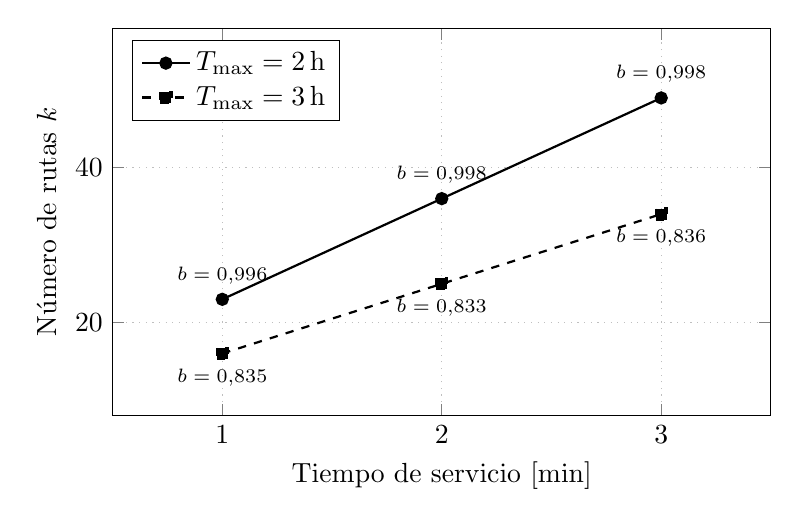
\begin{tikzpicture}
    \begin{axis}[
      width=0.82\textwidth,
      height=6.5cm,
      xlabel={Tiempo de servicio [min]},
      ylabel={Número de rutas $k$},
      xtick={1,2,3},
      xmin=0.5, xmax=3.5,
      ymin=8, ymax=58,
      legend pos=north west,
      grid=major,
      grid style={dotted,gray!50},
    ]
      \addplot[mark=*,thick,solid] coordinates {
        (1,23) (2,36) (3,49)
      };
      \addlegendentry{$T_{\max}=2$\,h}

      \addplot[mark=square*,thick,dashed] coordinates {
        (1,16) (2,25) (3,34)
      };
      \addlegendentry{$T_{\max}=3$\,h}

      \node[above=2pt] at (axis cs:1,23) {\scriptsize $b=0{,}996$};
      \node[above=2pt] at (axis cs:2,36) {\scriptsize $b=0{,}998$};
      \node[above=2pt] at (axis cs:3,49) {\scriptsize $b=0{,}998$};

      \node[below=2pt] at (axis cs:1,16) {\scriptsize $b=0{,}835$};
      \node[below=2pt] at (axis cs:2,25) {\scriptsize $b=0{,}833$};
      \node[below=2pt] at (axis cs:3,34) {\scriptsize $b=0{,}836$};
    \end{axis}
  \end{tikzpicture}
  \caption{Compromiso entre flota ($k$) y balance ($b$) según el tiempo de servicio y la cota
  $T_{\max}$.}
  \label{fig:grilla-spatial-k}
\end{figure}

\subsubsection*{Alcance de las comparaciones y decisión}

Las tres estrategias se comparan exclusivamente dentro del \textit{head-to-head} de la
Tabla~\ref{tab:estrategias}, que es el único contraste homogéneo disponible: mismo código, mismo
presupuesto de \textit{solver} y mismas semillas. La grilla de seis variantes del perfil de
rendimiento (Sección~\ref{sec:perfil-rendimiento}, Tabla~\ref{tab:grilla-variantes}) proviene de un
régimen de medición distinto ---estrategia \texttt{global}, código previo a la corrección del
redondeo del tránsito y límite de \textit{solver} de 180\,s--- y por tanto no es comparable arco a
arco con la Tabla~\ref{tab:grilla-spatial}: cualquier diferencia entre ambas estaría confundida
entre tres causas simultáneas (estrategia, redondeo y presupuesto de tiempo). Se la conserva porque
sus hallazgos de \textit{tiempo} ---la dominancia del GLS y el carácter \textit{OSRM-bound} en
frío--- no dependen de ninguno de esos tres factores.

El valor del coeficiente \texttt{SPATIAL\_SPAN\_COEF} se sometió a un barrido posterior sobre los
valores $\{0,\,3,\,10,\,30\}$, con tres semillas por punto y las doce instancias congeladas del
\hyperref[anx:suite-instancias]{Anexo 4}. Su resultado no habilita ningún valor mejor que el de
fábrica, pero tampoco lo confirma como óptimo: sobre la instancia de referencia los auto-cruces
sobre calle no varían de forma monótona con el coeficiente ---$39{,}7$ sin penalización espacial,
$34{,}3$ en el valor de producción, y $46{,}0$ y $48{,}0$ al subirlo a $10$ y a $30$---, de modo que
la mejora que el valor de producción obtiene sobre no penalizar, de un $13{,}6$\,\%, queda lejos del
criterio de decisión y se revierte en cuanto el coeficiente crece. La lectura obliga además a una
reserva sobre lo que la estrategia compra: en esa misma instancia, suprimir la penalización espacial
entrega mejor tiempo de desplazamiento ($57\,352$\,s frente a $58\,948$\,s) y mejor balance ($0{,}874$
frente a $0{,}839$). Lo que \texttt{spatial\_term} compra es compacidad y menor solapamiento entre
rutas, y lo paga en tiempo y en balance; no es una mejora en todos los ejes a la vez. El único eje
con señal pendiente ---el IoU del peor par--- es, como se argumentó, un problema de geometría local
que un coeficiente global no separa sin penalizar al resto de las rutas. La decisión que se
desprende del experimento es, en consecuencia, adoptar \texttt{spatial\_term} como estrategia por
defecto del sistema, con \texttt{SPATIAL\_SPAN\_COEF} $=3$, un límite de \textit{solver} de 120\,s
y la configuración censal de referencia de 2\,min de servicio con $T_{\max}=3$\,h;
\texttt{cluster\_first} se mantiene disponible como opción de comparación, pero no como
\textit{default} de producción. El protocolo completo, los comandos reproducibles y los datos crudos
de este experimento se encuentran versionados en \texttt{docs/experiments/} (reportes
\texttt{route-quality-20260712.md} y \texttt{spatial-span-20260730.md}, con los archivos CSV
asociados).

% ---- 4.1.4 ------------------------------------------------------
\subsection{Evaluación sobre áreas reales de censo y precio de la partición}
\label{sec:areas-reales}

Las comparaciones anteriores se ejecutaron sobre el conjunto de evaluación de $n = 1\,607$ árboles,
que reúne el arbolado de las dos bases legadas en una sola instancia. Los árboles que lo componen
son reales, pero la agrupación carece de correlato operativo, dado que el censo histórico se
organizó por área. Queda entonces sin responder la pregunta que la operación plantea de forma
directa: qué obtiene un censo real cuando el problema se entrega en su escala natural ---un área
individual de extensión $\leq 1{,}32$\,km--- en lugar de la unión de varias. Este apartado la
responde con una medición propia y, además, pone precio a la partición misma.

\subsubsection*{Instancias y brazos}

Se emplearon las tres áreas del censo histórico con mayor arbolado y su unión, congeladas como
instancias versionadas en \texttt{docs/experiments/instances/}. Las tres áreas son disjuntas por
identidad de árbol ---intersección vacía en las tres parejas sobre la clave \texttt{(source,
external\_id)}, con $157 + 72 + 43 = 272$ igual al cardinal de la unión---, de modo que la unión y
la suma de las partes resuelven exactamente el mismo arbolado. La Tabla~\ref{tab:areas-instancias}
las describe; el diámetro es la mayor distancia de \textit{haversine} entre dos árboles de la
instancia.

\begin{table}[H]
  \centering
  \caption{Instancias de área real y su unión, con el diámetro de cada una.}
  \label{tab:areas-instancias}
  \begin{tabularx}{\textwidth}{lXX}
    \toprule
    Instancia &
      $n$ &
      Diámetro \\
    \midrule
    \texttt{area-26-n157}         &
      157 &
      $1\,349$\,m \\
    \texttt{area-27-n72}          &
      72  &
      $979$\,m \\
    \texttt{area-29-n43}          &
      43  &
      $417$\,m \\
    \texttt{areas-26-27-29-n272}  &
      272 &
      $2\,685$\,m \\
    \bottomrule
  \end{tabularx}
\end{table}

Sobre cada instancia se ejecutaron tres brazos. El primero es la configuración de producción de
\textit{OR-Tools} ---estrategia \texttt{spatial\_term}, post-proceso 2-opt activo
(Sección~\ref{sec:postpass}), presupuesto de \textit{solver} de 120\,s, $T_{\min} = 7\,200$\,s,
$T_{\max} = 10\,800$\,s y 2\,min de servicio--- con tres semillas. El segundo es el
\textit{baseline} \textit{greedy} de vecino más cercano de la Sección~\ref{sec:comparacion-greedy},
determinista. El tercero es ese mismo \textit{baseline} con el post-proceso 2-opt aplicado a su
salida. El tercer brazo existe porque contrastar el método propio con refinamiento contra un
competidor sin refinamiento mide el post-proceso y no el \textit{solver}: el 2-opt reduce el
desplazamiento del \textit{greedy} un $6{,}7$\,\%, $22{,}5$\,\%, $4{,}6$\,\% y $1{,}7$\,\% en las
cuatro instancias, de manera que omitirlo habría inflado la ventaja aparente del \textit{solver}
entre $1{,}6$ y $35$ puntos porcentuales según la instancia. Es la misma asimetría de tratamiento
que la comparación de la Sección~\ref{sec:comparacion-greedy} arrastra sobre $n = 1\,607$ y que allí
queda como reserva declarada.

El criterio de decisión se fijó y versionó antes de ejecutar el experimento: el \textit{solver} gana
si, en las tres áreas y contra el tercer brazo, su desplazamiento no supera al del \textit{greedy}
refinado o lo empeora en a lo más un 5\,\%, ninguna de sus rutas queda sobre el 95\,\% de $T_{\max}$
y su balance alcanza al menos $0{,}80$. El margen se fijó en desplazamiento y saturación, nunca en
auto-cruces, por la reserva de instrumento que documenta la Sección~\ref{sec:discusion-calidad}. Se
declaró también que un estrechamiento o una inversión del margen se publicaría igual.

\subsubsection*{Resultados por área}

La Tabla~\ref{tab:areas-brazos} reúne los tres brazos. Las cifras de \textit{OR-Tools} son la media
de las tres semillas. La saturación máxima es la duración de la ruta más larga dividida por
$T_{\max}$. Ningún brazo dejó árboles sin asignar ni produjo rutas sobre $T_{\max}$.

\begin{table}[H]
  \centering
  \caption{
    Comparación de \textit{OR-Tools}, \textit{greedy} crudo y \textit{greedy} con 2-opt sobre las
    áreas reales y su unión (desplazamiento en segundos).
  }
  \label{tab:areas-brazos}
  \begin{tabularx}{\textwidth}{lXrrrl}
    \toprule
    Instancia &
      Brazo &
      $k$ &
      Desplaz. &
      Balance &
      Sat. máx. \\
    \midrule
    \texttt{area-26-n157} &
      \textit{OR-Tools}      &
      3 &
      $4\,859$ &
      $0{,}872$ &
      $0{,}77$--$0{,}82$ \\
    \texttt{area-26-n157} &
      \textit{greedy}        &
      3 &
      $5\,900$ &
      $0{,}301$ &
      $0{,}998$ \\
    \texttt{area-26-n157} &
      \textit{greedy} + 2-opt& 3 &
      $5\,502$ &
      $0{,}276$ &
      $0{,}993$ \\
    \midrule
    \texttt{area-27-n72}  &
      \textit{OR-Tools}      &
      2 &
      $2\,466$ &
      $0{,}887$ &
      $0{,}53$--$0{,}56$ \\
    \texttt{area-27-n72}  &
      \textit{greedy}        &
      1 &
      $2\,024$ &
      $1{,}000$ &
      $0{,}987$ \\
    \texttt{area-27-n72}  &
      \textit{greedy} + 2-opt& 1 &
      $1\,569$ &
      $1{,}000$ &
      $0{,}945$ \\
    \midrule
    \texttt{area-29-n43}  &
      \textit{OR-Tools}      &
      1 &
      $984$ &
      $1{,}000$ &
      $0{,}57$ \\
    \texttt{area-29-n43}  &
      \textit{greedy}        &
      1 &
      $1\,007$ &
      $1{,}000$ &
      $0{,}571$ \\
    \texttt{area-29-n43}  &
      \textit{greedy} + 2-opt& 1 &
      $961$ &
      $1{,}000$ &
      $0{,}567$ \\
    \midrule
    \texttt{areas-26-27-29-n272} &
      \textit{OR-Tools}       &
      5 &
      $9\,462$ &
      $0{,}896$ &
      $0{,}82$--$0{,}83$ \\
    \texttt{areas-26-27-29-n272} &
      \textit{greedy}         &
      5 &
      $9\,856$ &
      $0{,}011$ &
      $0{,}993$ \\
    \texttt{areas-26-27-29-n272} &
      \textit{greedy} + 2-opt &
      5 &
      $9\,691$ &
      $0{,}011$ &
      $0{,}992$ \\
    \bottomrule
  \end{tabularx}
\end{table}

El criterio se cumple en dos de las tres áreas. En \texttt{area-26-n157} el \textit{solver} gana con
holgura: reduce el desplazamiento un $11{,}7$\,\% respecto del \textit{greedy} refinado, alcanza un
balance de $0{,}872$ frente a $0{,}276$ y ninguna de sus rutas supera el 82\,\% de $T_{\max}$. El
\textit{baseline} reparte los 157 árboles en rutas de 74, 72 y 11 paradas, esto es, dos jornadas al
$99{,}3$\,\% y al $98{,}7$\,\% de $T_{\max}$ y un muñón de $2\,962$\,s, mientras que el
\textit{solver} produce jornadas de $8\,275$, $8\,042$ y $7\,460$\,s. Es el caso que el criterio
anticipaba: la ventaja del método no se agota en el desplazamiento, sino en que entrega jornadas
ejecutables.

En \texttt{area-29-n43} el criterio también se cumple, aunque de forma poco informativa. El
\textit{solver} empeora el desplazamiento un $2{,}4$\,\%, dentro del margen declarado del 5\,\%, con
$k=1$ en ambos métodos y la misma jornada de aproximadamente $6\,100$\,s. Con 43 árboles la
instancia es demasiado pequeña para distinguir métodos: ambos resuelven el mismo recorrido único.

En \texttt{area-27-n72} el criterio falla, y por un margen amplio. El \textit{greedy} refinado cubre
los 72 árboles en una sola jornada de $10\,209$\,s ---el $94{,}5$\,\% de $T_{\max}$--- con
$1\,569$\,s de desplazamiento, mientras que el \textit{solver} abre dos rutas de $5\,766$ y
$5\,597$\,s y gasta $2\,466$\,s, un $57$\,\% más de caminata y dos medias jornadas en lugar de una
completa. No hay aquí ruta degenerada que reprochar al \textit{baseline}: su solución es la que un
censador preferiría. Como el criterio exigía las tres áreas, el veredicto global frente al
pre-registro es de incumplimiento, y así se reporta.

\subsubsection*{El caso \texttt{area-27} es el régimen de relleno por $T_{\min}$}

El resultado adverso admite un diagnóstico preciso, pero no el de un fallo de búsqueda: es el
régimen de relleno que la Sección~\ref{sec:discusion-calidad} caracteriza más adelante para
instancias que no saturan su presupuesto temporal. Con la configuración de producción las cotas
blandas no dependen de la instancia: el método \texttt{PenaltyConfig.vehicle\_bounds} devuelve, para
las cuatro instancias de este apartado, un piso en $T_{\min} = 7\,200$\,s con coeficiente
$10\,000\,\text{s}^{-1}$ y un objetivo superior en el punto medio de $9\,000$\,s con coeficiente
$500\,\text{s}^{-1}$.

Instrumentar directamente el valor de la función objetivo del \textit{solver} en esta instancia
---inyectando la solución del \textit{greedy} como \textit{warm start} y comparando su costo contra
el de la solución final de partición (\texttt{warmstart-area27-20260730.csv})--- muestra que las
duraciones de las dos rutas que reporta \texttt{total\_estimated\_time\_sec} no son el valor que ve
la dimensión Time del \textit{solver}. Esas duraciones son $5\,766$ y $5\,597$\,s en la corrida de
esta sección, y $5\,299$ y $5\,819$\,s en la repetición instrumentada; la diferencia con la
dimensión Time es relleno de trayecto añadido gratis, y ambas rutas terminan exactamente en el piso
$T_{\min} = 7\,200$\,s. Con esa cifra la partición no paga penalización de piso, $(7\,200 - 7\,200)
\times 10\,000 = 0$ por vehículo, y su costo se reduce al fijo de dos vehículos, $200\,000$. La
jornada única del \textit{greedy}, en cambio, paga $(10\,694 - 9\,000) \times 500 = 847\,000$ de
exceso sobre el objetivo superior más $100\,000$ de costo fijo; los $10\,694$\,s son la duración de
la solución inyectada, que es la variante cruda del \textit{greedy}, y no los $10\,209$\,s de su
variante con 2-opt de la Tabla~\ref{tab:areas-brazos}. El valor de la función objetivo lo confirma:
$964\,903$ para la jornada única inyectada como \textit{warm start} frente a $229\,709$ para la
partición que devuelve el \textit{solver}, un factor cercano a $4{,}2$ a favor de partir. El
\textit{solver} la devuelve, en efecto, en las tres semillas, con y sin \textit{warm start} de la
jornada única. No hay óptimo local que reprochar a la búsqueda: el GLS encontró y conservó la
solución más barata bajo el precio vigente.

El mecanismo es el mismo régimen de relleno por $T_{\min}$ documentado en la
Sección~\ref{sec:discusion-calidad}: cuando $k \cdot T_{\min}$ excede holgadamente el trabajo real
de la instancia ---aquí $2 \times 7\,200 = 14\,400$\,s frente a los $10\,694$\,s que exige recorrer
los 72 árboles en una sola ruta---, partir y rellenar hasta el piso resulta más barato que una única
ruta que se pasa del objetivo superior. La palanca para este defecto ya se intentó por la vía de los
pisos (piso de paradas, piso combinado) y quedó cerrada sin cambio de \textit{default}: no es un
hueco de búsqueda nuevo que abra un ciclo de precios adicional.

Las restantes instancias son consistentes con estos mismos precios. En \texttt{area-26} el
\textit{solver} deja sus tres rutas dentro de la banda $[7\,200,\ 9\,000]$, donde no se paga nada, y
en la unión la ruta más larga de cada semilla se queda en el $82$--$83$\,\% de $T_{\max}$, esto es,
por debajo de los $9\,000$\,s del objetivo superior, con duraciones medias por semilla de $8\,204$,
$8\,121$ y $8\,936$\,s. \texttt{area-29} es el caso sin salida: 43 árboles no alcanzan para
$7\,200$\,s, así que su única ruta paga el piso porque no existe alternativa. Ni la búsqueda ni la
recalibración de coeficientes son la palanca pertinente aquí: ambas vías ---piso de paradas, piso
combinado, recalibración de penalizaciones--- ya fueron exploradas y descartadas por otras razones
(Sección~\ref{sec:discusion-calidad}).

\subsubsection*{Precio de particionar}

El segundo contraste enfrenta la unión de las tres áreas contra la suma de resolverlas por separado.
Se pre-registró que particionar costaría kilómetros, por prohibir rutas que crucen el borde entre
áreas, y que ganaría tratabilidad. La medición sale al revés en el eje de desplazamiento y se
reporta igual. La Tabla~\ref{tab:precio-particion} enfrenta ambas magnitudes.

\begin{table}[H]
  \centering
  \caption{Unión de las tres áreas frente a la suma de resolverlas por separado.}
  \label{tab:precio-particion}
  \begin{tabularx}{\textwidth}{lXX}
    \toprule
    Magnitud &
      Suma por área &
      Unión \texttt{n272} \\
    \midrule
    Desplazamiento medio (3 semillas) &
      $8\,309$\,s &
      $9\,462$\,s \\
    Desplazamiento mediano            &
      $8\,272$\,s &
      $8\,381$\,s \\
    Número de rutas $k$               &
      $3 + 2 + 1 = 6$ &
      $5$ \\
    Balance                           &
      $0{,}872$ / $0{,}887$ / $1{,}000$ &
      $0{,}896$ \\
    Saturación media                  &
      $0{,}732$ / $0{,}514$ / $0{,}569$ &
      $0{,}780$ \\
    Rutas bajo $T_{\min}$             &
      $0$ / $2$ / $1$ &
      $0$ \\
    Cómputo total (3 semillas)        &
      $3 \times 3 \times 120$\,s $= 1\,080$\,s &
      $3 \times 120$\,s $= 360$\,s \\
    \bottomrule
  \end{tabularx}
\end{table}

Particionar no cuesta desplazamiento en este territorio. Las tres áreas están separadas ---diámetros
de $1\,349$, $979$ y $417$\,m frente a $2\,685$\,m de la unión---, de modo que apenas existe ruta
que gane cruzando el borde entre ellas, y la ventaja de la unión no es geométrica sino de llenado:
con 272 árboles el \textit{solver} arma cinco jornadas de aproximadamente $8\,400$\,s en lugar de
seis de unos $6\,800$\,s, de las cuales tres quedarían bajo $T_{\min}$.

La ventaja aparente de la partición en desplazamiento medio ---un $12{,}2$\,\% menos--- exige una
reserva: descansa casi entera en una semilla: la unión resuelve en $8\,381$, $7\,964$ y $12\,040$\,s
según la repetición, un $51$\,\% de dispersión, y con la mediana la diferencia cae a un $1{,}3$\,\%.
La lectura que el material sostiene es que, al mismo presupuesto por corrida, la instancia
monolítica resulta menos estable, y no que particionar ahorre caminata. Ese presupuesto por corrida,
además, no es comparable en total: la partición consumió el triple de cómputo.

El precio medido de particionar es, entonces, una jornada de censador más, tres jornadas por debajo
de $T_{\min}$ y el triple de cómputo, a cambio de instancias de aproximadamente $1{,}3$\,km que
corresponden a una unidad operativa real y de una varianza entre repeticiones sustancialmente menor.
Los auto-cruces y el solapamiento entre rutas se registraron como contexto y no formaron parte del
criterio de este ciclo.

Este resultado convierte en medición lo que la Sección~\ref{sec:discusion-calidad} argumentaba desde
la geometría. La segmentación previa por área, que la Sección~\ref{sec:posibles-mejoras} documenta
como trabajo futuro, deja de sostenerse solo en que el régimen disperso produce auto-cruces y pasa a
tener un costo cuantificado ---una ruta adicional, jornadas cortas y triple cómputo--- frente a un
beneficio también cuantificado, a saber, instancias con correlato operativo y menor varianza. El
protocolo, los comandos reproducibles y los datos crudos se encuentran versionados en
\texttt{docs/experiments/} (reporte \texttt{area-partition-20260726.md} y los archivos CSV
asociados).

% ---- 4.1.5 ------------------------------------------------------
\subsection{Discusión de calidad de rutas}
\label{sec:discusion-calidad}

La función objetivo que minimiza el \textit{solver} combina seis componentes de escala diferente
(Ecuación~\ref{eq:objetivo}). El término principal es el costo de arco, proporcional al tiempo de
tránsito entre paradas consecutivas (aproximadamente 1\,s por segundo de caminata según la red
peatonal de OSRM). Sobre él actúan dos penalizaciones blandas en la dimensión temporal de cada ruta:
la penalización inferior, con coeficiente $10\,000\,\text{s}^{-1}$, desalienta que una ruta quede
por debajo de $T_{\min}$; y la penalización superior, con coeficiente $500\,\text{s}^{-1}$,
desalienta que la duración supere el punto medio del intervalo $[T_{\min},\,T_{\max}]$. Se añaden
además un costo fijo de $100\,000$\,s por vehículo activo, que desincentiva el uso de rutas
adicionales, y una penalización de $1\,000\,000$\,s por árbol no cubierto, que garantiza que la
cobertura total sea siempre preferible a cualquier mejora marginal en los demás términos. El sexto
componente es el costo de extensión geográfica, con coeficiente $\lambda_{\text{span}} = 3$ por
metro de \textit{span} \textit{haversine} de cada ruta, que solo actúa bajo la estrategia
\texttt{spatial\_term} y es lo que la distingue de \texttt{global}.

La razón entre ambas penalizaciones blandas es de $20\mathord{:}1$ ($10\,000 / 500$), y el
experimento de sensibilidad a los coeficientes de penalización ---cuyos datos se conservan en
\texttt{docs/experiments/penalty-sensitivity-20260713-reference.csv}--- ofrece evidencia causal de
la función que cumple cada término. Al suprimir la penalización inferior (coeficiente $= 0$),
manteniendo fijo el resto de los coeficientes, el balance de carga cae de $0{,}838$ a $0{,}739$, la
flota sube de 25 a 32 rutas y el número de rutas que quedan por debajo de $T_{\min}$ pasa de 3 a 26,
lo que confirma que ese componente es el mecanismo que sostiene la distribución de carga y evita la
fragmentación en rutas demasiado cortas.

La penalización superior actúa sobre la geometría: al redirigir su objetivo desde el punto medio del
intervalo hasta $T_{\max}$, el número de auto-cruces medido sobre cuerdas cae de $76{,}3$ a $6{,}3$
---una reducción del $91{,}7$\,\%--- sin variar el presupuesto de cómputo ni el número de rutas. Esa
cifra no sostiene, sin embargo, una relación causal directa: el barrido no tiene réplicas de semilla
independientes, la métrica de cuerdas está invertida ($\rho = -0{,}575$) precisamente en la
instancia donde se midió, y el mismo brazo degrada el balance de $0{,}838$ a $0{,}715$. El
\hyperref[anx:reservas-sensibilidad]{Anexo 4} detalla las tres reservas. Con ellas, lo que el
material sostiene es evidencia consistente con la hipótesis de que la geometría de las rutas
responde a la configuración de la función objetivo y no al corte por tiempo del GLS, reforzada por
dos observaciones independientes: el presupuesto del \textit{solver} no altera el número de rutas ni
el balance por sobre los 120\,s (Tabla~\ref{tab:sensibilidad-tl}), y la re-medición sobre
\texttt{crossings\_road} invierte el signo del efecto de este mismo brazo sobre la geometría real.

El significado de ese diagnóstico depende del régimen geográfico del \textit{dataset}. El conjunto
de evaluación de $n = 1\,607$ árboles agrega arbolado real de múltiples áreas de censo dispersas en
$\approx 10{,}3$\,km de extensión ($12{,}5$\,km de diagonal), frente a $1{,}32$\,km del área
individual mayor ---razón cercana a $8\times$, según las instancias versionadas en
\texttt{docs/experiments/instances/}---. Los árboles son reales; lo sin correlato operativo es
tratar esa unión ---las veintiuna áreas no vacías de \texttt{legacy\_api} (429 árboles, 27\,\% del
conjunto) más los 1\,178 árboles de \texttt{legacy\_app}, sin área asignada--- como un único trabajo
de ruteo (Ilustración~\ref{fig:regimen-disperso-vs-real}). En el régimen de área real la
configuración de producción genera rutas sin auto-cruces apreciables; estos emergen solo al procesar
el conjunto agregado disperso bajo la estrategia \texttt{spatial\_term}
(Ilustración~\ref{fig:ruta-vueltas-r1}), situación que en operación solo surgiría si se procesaran
múltiples áreas de censo como un único problema.

\begin{figure}[H]
  \centering
  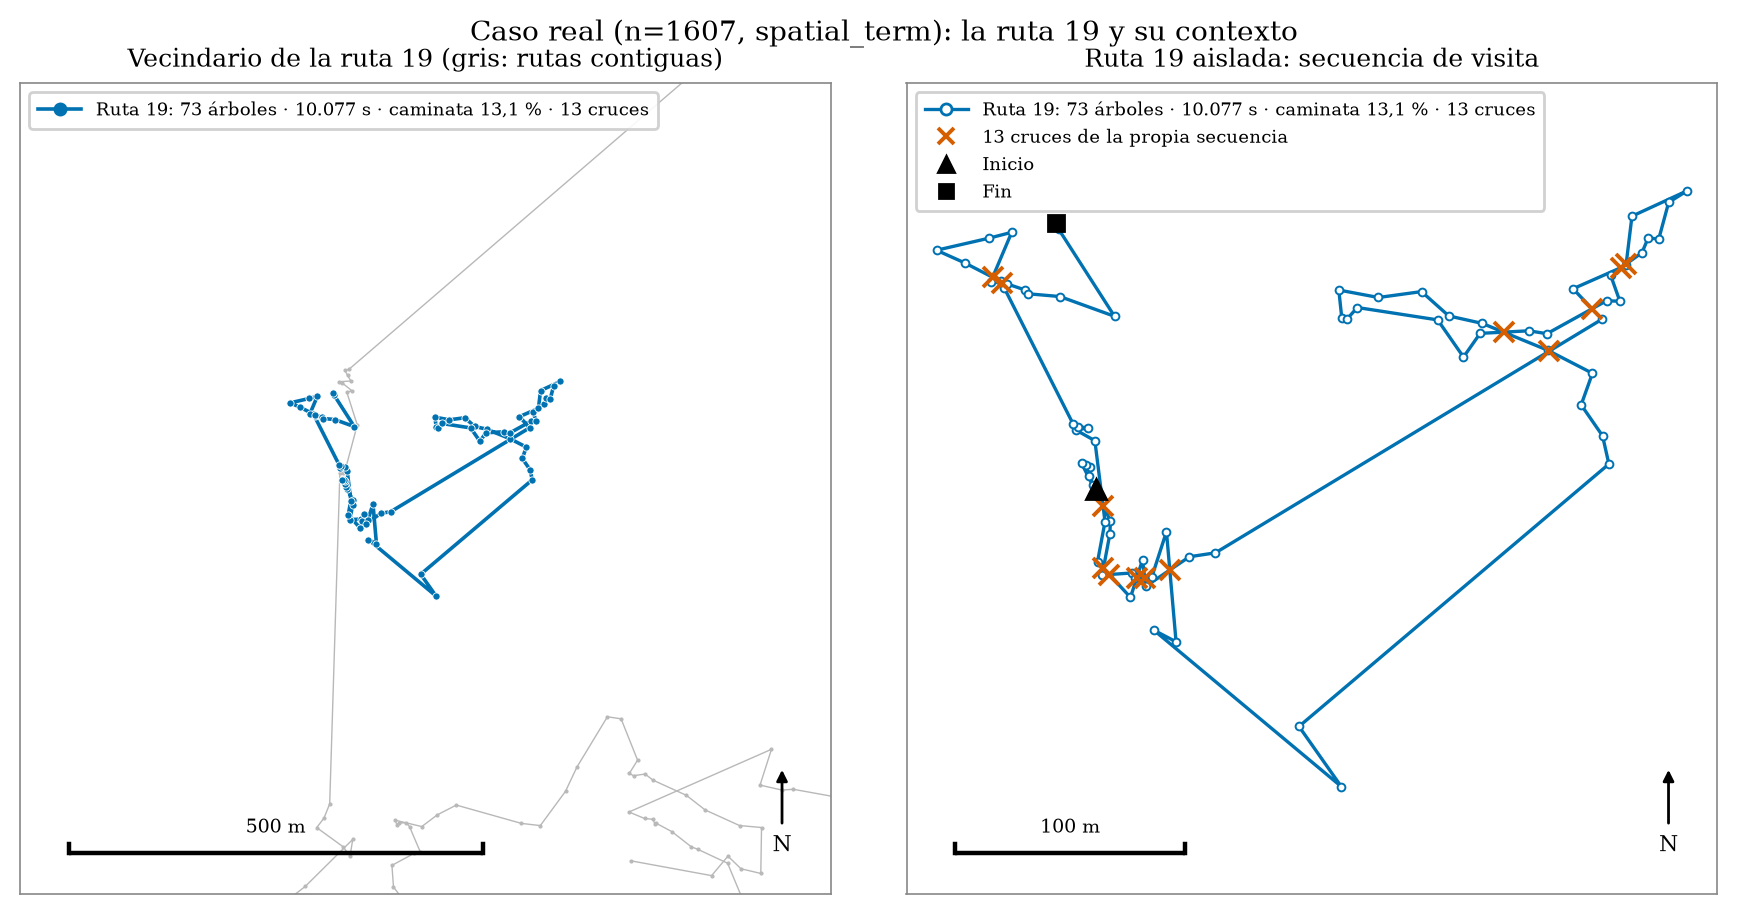
\includegraphics[width=0.9\textwidth]{media/fig-ruta-vueltas-r1.png}
  \caption{Ruta con auto-cruces en el \textit{dataset} de evaluación.}
  \label{fig:ruta-vueltas-r1}
\end{figure}

La diferencia entre ambos regímenes se aprecia en la extensión que abarca cada uno:
$\approx 10{,}3$\,km en el conjunto agregado frente a $\leq 1{,}32$\,km en las áreas individuales.

\begin{figure}[H]
  \centering
  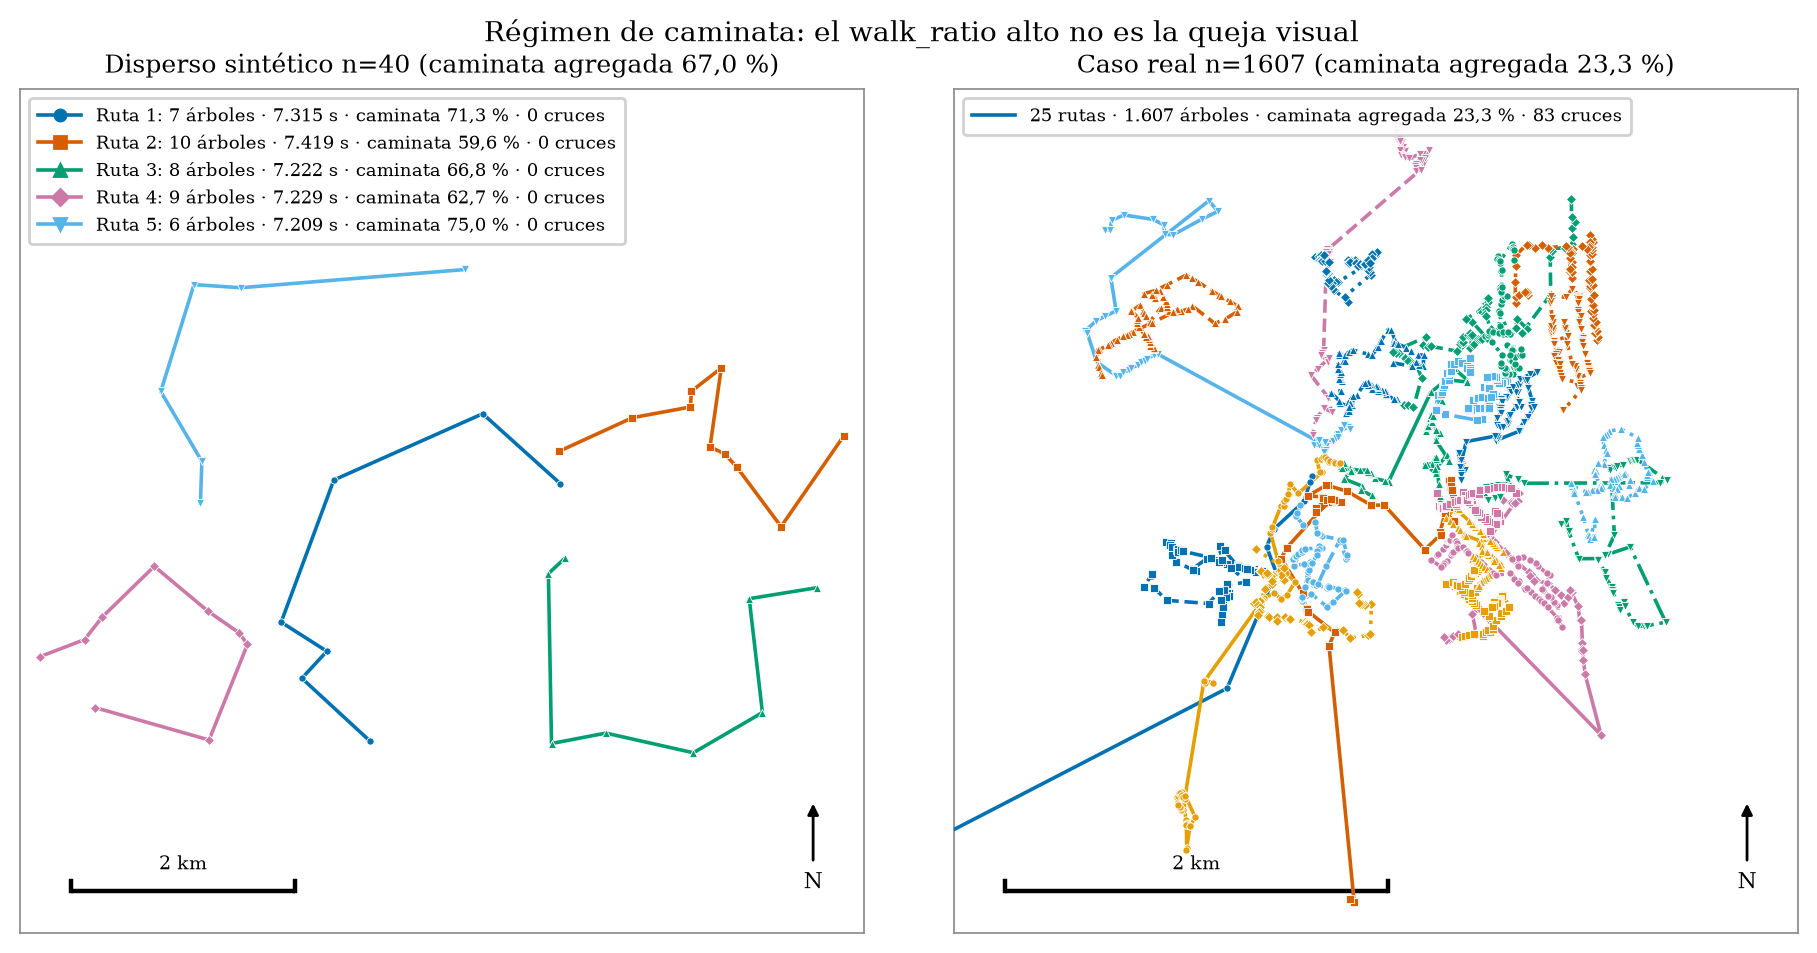
\includegraphics[width=0.9\textwidth]{media/fig-regimen-disperso-vs-real.png}
  \caption{
    Régimen disperso (\textit{dataset} de evaluación agregado) frente a régimen real (áreas
    individuales del arbolado legado).
  }
  \label{fig:regimen-disperso-vs-real}
\end{figure}

El peor par de rutas anunciado en la Sección~\ref{sec:comparacion-estrategias}, con un \textit{IoU}
de $0{,}55$, se reproduce en la Ilustración~\ref{fig:peor-par}.

\begin{figure}[H]
  \centering
  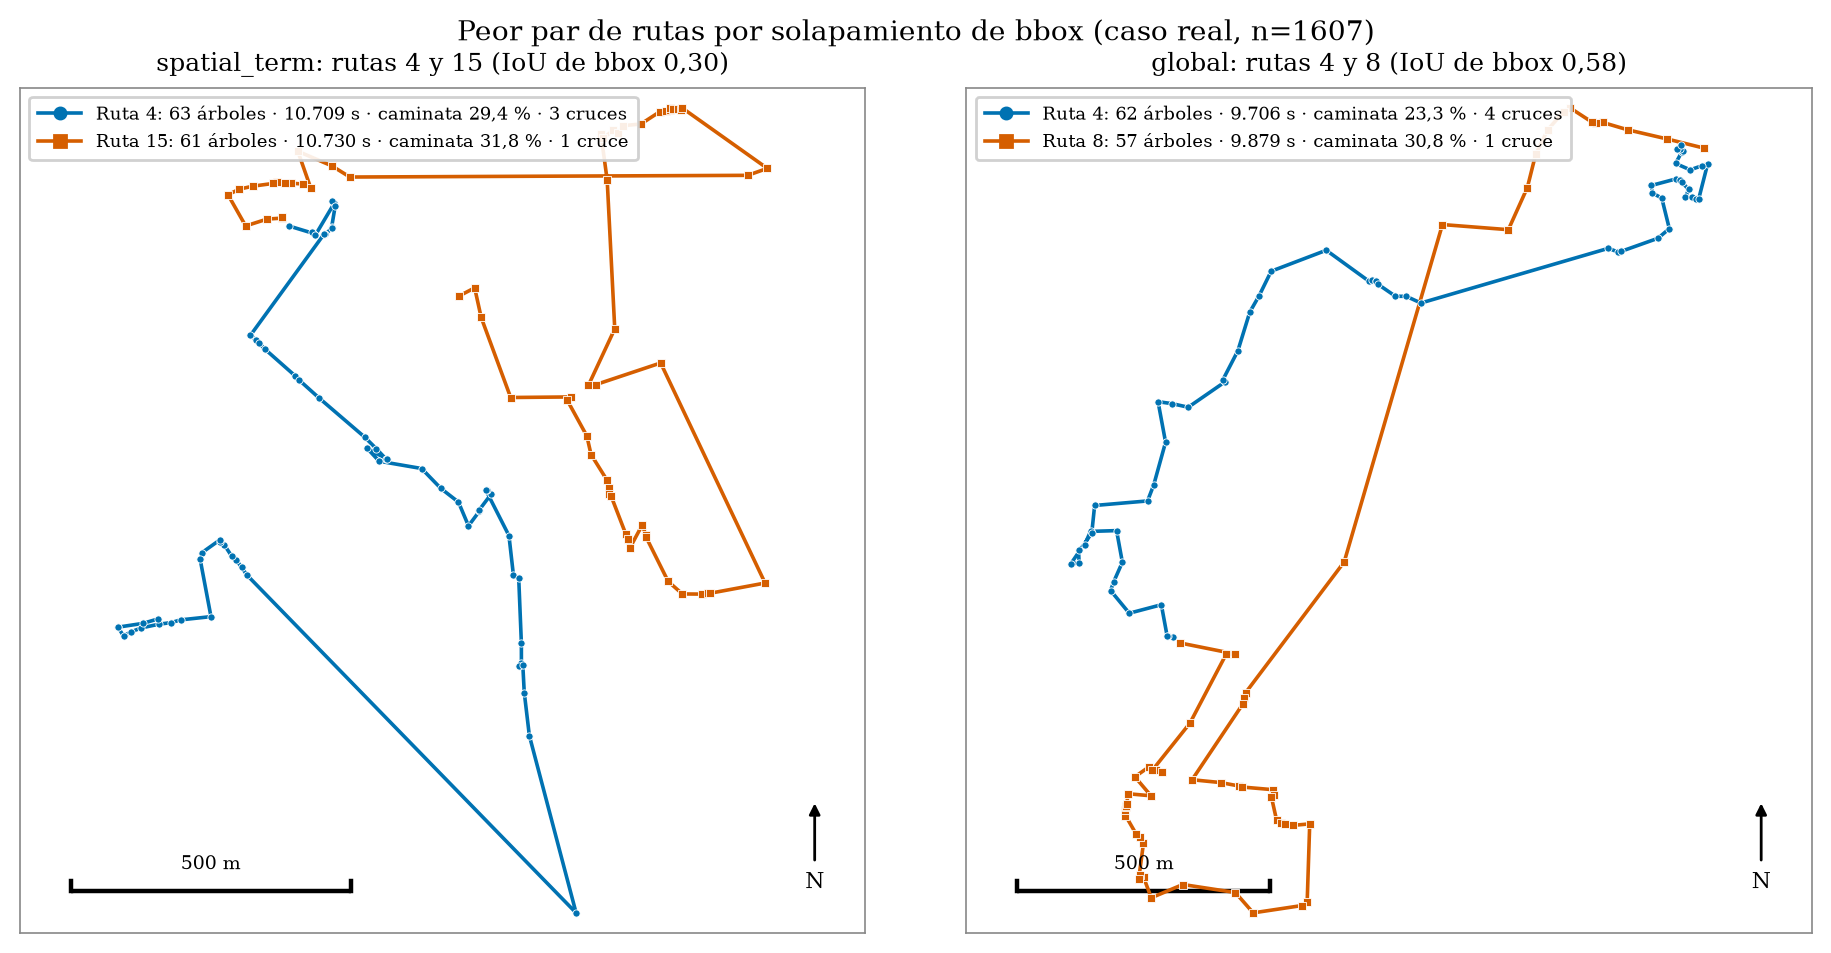
\includegraphics[width=0.9\textwidth]{media/fig-peor-par.png}
  \caption{Par de rutas con mayor solapamiento espacial en el \textit{dataset} de evaluación.}
  \label{fig:peor-par}
\end{figure}

El solapamiento persiste con la estrategia \texttt{spatial\_term} porque responde a la geometría
local del par, y ningún coeficiente global lo elimina sin penalizar las rutas circundantes; la
solución estructural es la segmentación previa por área de censo.

De los resultados anteriores se derivan dos respuestas directas a las preguntas de evaluación más
frecuentes. La pregunta «¿por qué las rutas no se ven compactas visualmente?» tiene respuesta en la
geometría: la configuración de producción produce rutas sin auto-cruces en áreas de extensión real
($\leq 1{,}32$\,km), y cuando los auto-cruces aparecen responden a la función objetivo, no a una
limitación del tiempo de cómputo. La pregunta «¿por qué el \textit{baseline} \textit{greedy} se
acerca en desplazamiento total?» tiene respuesta en la saturación: el heurístico llena cada ruta
hasta un $98$\,\% de $T_{\max}$ ---sin dejar holgura operacional--- de modo que su reducción de
caminata proviene de la cota, no de la calidad del ordenamiento. La diferencia de $4{,}7$\,\% de
desplazamiento a favor del \textit{solver} ---medida contra un \textit{baseline} que recibe el mismo
post-proceso de 2-opt--- y la menor severidad de su ruta residual son las dimensiones que el tiempo
total de desplazamiento no captura de forma aislada (Sección~\ref{sec:comparacion-estrategias}).

La unidad operativa del motor es el área de censo individual, no el arbolado metropolitano en su
conjunto. Procesar cada área como un problema independiente reduciría la extensión del
\textit{dataset} a la escala en que el \textit{solver} produce rutas limpias con la configuración
actual; esa extensión se documenta como trabajo futuro en la Sección~\ref{sec:posibles-mejoras} y su
costo se midió después sobre las áreas reales (Sección~\ref{sec:areas-reales}), donde resulta ser
una ruta adicional y el triple de cómputo, no kilómetros de caminata. El problema que esa extensión
plantea ---repartir un territorio en distritos compactos y equilibrados antes de rutear--- tiene
tratamiento propio en la literatura bajo la denominación de diseño territorial
\citep{kalcsics2005towards,rios2009reactive}, cuyos criterios de compacidad y de balance coinciden
con los dos ejes que esta sección mide.

Con el fin de confirmar el origen de los auto-cruces en la función objetivo y explorar si existe una
configuración universal, se ejecutó un barrido de configuración $\times$ algoritmo $\times$ tamaño
sobre las doce instancias reales congeladas del \hyperref[anx:suite-instancias]{Anexo 4} ($n=43$ a
$n=1\,607$). El único brazo que satisface el criterio de decisión sobre $n=1\,607$
---\texttt{upper-tmax-tmin9000}, que ancla la penalización blanda superior en $T_{\max}$ y eleva el
piso blando--- reduce los auto-cruces un $92{,}5$\,\% sin costo de viaje ni de balance en esa
instancia, porque a esa densidad las rutas saturan $T_{\max}$ de forma natural
($\overline{\text{sat}} = 0{,}94$). El mismo brazo produce, sin embargo, el peor resultado sobre las
áreas reales individuales, donde la instancia no satura $T_{\max}$: fuerza relleno de trayecto con
incrementos de viaje de hasta $+89$\,\%. Los brazos restantes no mejoran el criterio (el término de
\textit{span} temporal queda por debajo del umbral exigido) o rompen el balance de carga en varias
instancias. El \hyperref[anx:barrido-configuraciones]{Anexo 4} detalla las ocho configuraciones
evaluadas, brazo por brazo, sobre las 96 celdas del barrido.

La conclusión del barrido es que no existe una configuración única ganadora para todos los regímenes
sin una compuerta previa: la hipótesis queda refutada. El escenario donde
\texttt{upper-tmax-tmin9000} gana ---el conjunto agregado de $n=1\,607$--- no tiene correlato
operativo en el censo histórico, que se organizó por área; representa en cambio el régimen de
escalamiento, un censo de cobertura mayor o el ruteo de una comuna completa como un solo problema.
La decisión adoptada es conservar la configuración de producción (\texttt{actual}) sin modificación
y publicar \texttt{upper-tmax-tmin9000} como propuesta verificada para un \textit{guard} por
saturación a priori ($\overline{\text{sat}} \gtrsim 0{,}9$): el código de los \textit{overrides}
queda en el árbol (opt-in, producción intacta) para habilitar ese \textit{guard} cuando se
implemente el selector, extensión que se documenta en la Sección~\ref{sec:posibles-mejoras}.

\subsubsection*{Auditoría de robustez metodológica}

La serie experimental registra dieciséis ciclos de evaluación cerrados durante julio de 2026. El
análisis retrospectivo identificó cuatro defectos de instrumentación en los ciclos iniciales
---semillas no propagadas, una cota de relleno inalcanzable, la métrica de auto-cruces sobre cuerdas
en lugar del trazado real, y un criterio de degeneración que mezclaba dos fenómenos distintos---,
que el \hyperref[anx:auditoria-robustez]{Anexo 4} detalla con el alcance necesario para reproducir
cada corrección.

Estas correcciones se originaron dentro de la propia serie y no invalidan sus conclusiones: de los
dieciséis ciclos, uno queda con el veredicto impugnado, dos se releyeron con el instrumento
corregido sin que cambiara el descarte final y los demás descansan en criterios ---tiempo de viaje,
relleno, balance--- ajenos a los defectos detectados. El caso de mayor alcance es el 2-opt
intra-ruta (Sección~\ref{sec:postpass}), rechazado en un ciclo de evaluación anterior por empeorar
los auto-cruces medidos en cuerdas: la auditoría de instrumento mostró que ese empeoramiento era
artefacto de la métrica y que el algoritmo limpia la geometría real, lo que revirtió el rechazo y lo
incorporó a la configuración de producción. Es el único cambio de configuración por defecto de toda
la serie, y no proviene de barrer términos de la función objetivo sino de corregir el instrumento de
medición.

\section{PERFIL DE RENDIMIENTO DEL OPTIMIZADOR}
\label{sec:perfil-rendimiento}

El tiempo de ejecución se concentra en la metaheurística cuando la caché de la matriz está caliente
---el GLS acapara el $98{,}1$\,\% del total--- y en OSRM cuando está fría. Esta sección documenta
ese comportamiento: en qué fases del \textit{pipeline} se concentra el tiempo de ejecución, cómo
varían las soluciones ante los parámetros operacionales (tiempo de servicio por árbol y cota dura
$T_{\max}$) y cuál es la sensibilidad del sistema al tamaño del problema y al presupuesto del
\textit{solver}. Todas las cifras provienen del experimento de perfilado ejecutado el 11--12 de
julio de 2026, cuyo protocolo y datos crudos se encuentran versionados en el directorio
\texttt{docs/experiments/} del repositorio (reporte \texttt{profiling-20260711.md} y archivos CSV
asociados), y son reproducibles mediante el comando de gestión \texttt{baseline\_sweep}, verificado
previamente sobre una corrida sintética de $n=80$ (\texttt{baseline-sweep-20260711.md}).

Corresponde advertir que las cifras de esta sección provienen de un régimen de medición anterior al
de la Sección~\ref{sec:comparacion-estrategias}: se obtuvieron con la estrategia \texttt{global}, un
límite de \textit{solver} de 180\,s y una versión del código previa a la corrección del redondeo del
tránsito (el truncamiento entero descrito al final de la Sección~\ref{sec:variantes-duracion}). Ese
era el régimen vigente en producción al momento del perfilamiento, y son sus propios resultados los
que lo dejaron obsoleto: la sensibilidad al límite de \textit{solver} es la que motivó bajarlo de
180 a 120\,s ---remedida sobre el código vigente en la Tabla~\ref{tab:sensibilidad-tl}---, mientras
que la adopción de \texttt{spatial\_term} como estrategia por defecto proviene del experimento de
comparación de la Sección~\ref{sec:comparacion-estrategias}. El perfil documenta, por tanto, el
estado previo a ambas decisiones y no se reejecutó bajo el régimen nuevo: sus tablas ---en
particular la grilla de seis variantes de la Tabla~\ref{tab:grilla-variantes}--- no deben cruzarse
arco a arco con las de la Sección~\ref{sec:comparacion-estrategias}, por las razones que allí se
detallan. La sección se conserva porque sus hallazgos son de \textit{tiempo} ---la dominancia del
GLS y el carácter \textit{OSRM-bound} en frío---, que no dependen de la estrategia ni del redondeo,
y porque el barrido de la Tabla~\ref{tab:sensibilidad-tl} trata el presupuesto de \textit{solver}
como variable del experimento y no como constante del régimen.

\subsection{Entorno de medición}

Dado que el sistema no cuenta con un despliegue productivo, las mediciones se realizaron sobre una
réplica local del entorno de producción definida en \texttt{docker-compose.prod.yml}. Esta réplica
usa imágenes construidas con el \textit{target} \texttt{prod} del \texttt{Dockerfile} (sin
\textit{bind-mounts} de código ni recarga en caliente, con usuario no privilegiado), una instancia
real de OSRM cargada con el extracto completo de Chile de \textit{OpenStreetMap}
(\texttt{chile-latest.osm.pbf}), preprocesado con el algoritmo \textit{Multi-Level Dijkstra}
\citep{delling2017customizable} y perfil peatonal, además de PostGIS \citep{postgis} 15--3.3 y Redis
7. Las versiones empleadas fueron Python 3.12.11, Django \citep{django} 6.0, \textit{OR-Tools}
\citep{ortools} 9.15 y NumPy 2.4.6.

Este entorno difiere de un despliegue real en tres condiciones que acotan la extrapolación de sus
cifras. El hardware es un Apple M4 Pro (arm64, 12 núcleos, 24\,GB) bajo Docker Desktop, con los
contenedores de base de datos y OSRM emulados en \texttt{linux/amd64} mediante Rosetta, mientras que
un servidor de producción típico sería x86 nativo con recursos menores. La comunicación con OSRM y
la base de datos ocurre, además, por la red interna de \textit{compose} en la misma máquina, con
latencia cercana a cero, mientras que en un centro de datos la latencia de red encarecería la fase
de consulta a OSRM (100 solicitudes HTTP para $n=1\,607$). Por último, el punto de entrada fue el
comando de gestión ejecutado secuencialmente dentro del contenedor, en lugar del flujo
API~$\rightarrow$~Celery del sistema en operación; ambos recorren el mismo código
(\texttt{OptimizationPipeline.run}), por lo que la diferencia agrega únicamente latencia de
encolado, no de cómputo.

\subsection{Desglose de tiempo por fase}

El \textit{pipeline} se instrumentó por fases: construcción de la matriz de costos
(\texttt{cost\_matrix}), construcción del modelo (\texttt{model\_build}), resolución
(\texttt{solve}, subdividida en primera solución y metaheurística), extracción de la solución
(\texttt{solution\_extraction}) y cálculo de métricas (\texttt{metrics}). El hallazgo central es que
el perfil depende del estado de la caché de la matriz de distancias: en operación normal (caché
caliente) el \textit{pipeline} está acotado por el \textit{solver} (\textit{solve-bound}), y solo en
el primer contacto con un \textit{dataset} está acotado por OSRM (\textit{OSRM-bound}).

Con la caché caliente, la metaheurística GLS concentra el 98,1\,\% del tiempo total, y todas las
demás fases combinadas representan menos del 2\,\% (Tabla~\ref{tab:fases-caliente}), media de las
18 corridas de la grilla. Optimizar la construcción del modelo, la extracción o el cálculo de
métricas no tendría, por tanto, ningún efecto medible.

\begin{table}[H]
  \centering
  \caption{Desglose de tiempo por fase con caché de matriz caliente.}
  \label{tab:fases-caliente}
  \begin{tabularx}{\textwidth}{lXX}
    \toprule
    Fase &
      Tiempo [s] &
      \% del total \\
    \midrule
    \texttt{cost\_matrix} (consulta de caché) &
      0{,}57 &
      0{,}5\,\% \\
    \texttt{model\_build} &
      $<0{,}01$ &
      $\approx 0$\,\% \\
    \texttt{solve} (primera solución) &
      1{,}4 &
      1{,}3\,\% \\
    \texttt{solve} (metaheurística GLS) &
      103{,}4 &
      98{,}1\,\% \\
    \texttt{solution\_extraction} &
      0{,}01 &
      $\approx 0$\,\% \\
    \texttt{metrics} &
      0{,}02 &
      $\approx 0$\,\% \\
    \midrule
    Total del \textit{pipeline} &
      105{,}4 &
      100\,\% \\
    \bottomrule
  \end{tabularx}
\end{table}

En frío ---caché de matriz vacía, primera corrida sobre el \textit{dataset}--- el perfil se
invierte: la consulta a OSRM domina con el 97,6\,\% del tiempo (Tabla~\ref{tab:fases-frio}), medido
en la corrida piloto con tiempo de servicio de 2\,min y $T_{\max}=3$\,h. Con $n=1\,607$ la
fragmentación por longitud de URL (175 coordenadas por bloque) convierte la matriz en una grilla de
$10 \times 10 = 100$ solicitudes al servicio \texttt{/table}, con un costo total de 170{,}8\,s que
escala aproximadamente como $O(n^2)$ con el número de celdas. La cifra difiere en un 4\,\% de la
corrida en frío citada en la Sección~\ref{sec:metricas-calidad}, dispersión propia de la latencia de
cien solicitudes HTTP sucesivas. Este costo se paga una única vez por \textit{dataset}: la matriz
queda almacenada en caché (indexada por el hash SHA-256 de los identificadores de árboles activos),
de modo que toda corrida posterior es \textit{solve-bound}.

\begin{table}[H]
  \centering
  \caption{Desglose de tiempo por fase en frío.}
  \label{tab:fases-frio}
  \begin{tabularx}{\textwidth}{lXX}
    \toprule
    Fase &
      Tiempo [s] &
      \% del total \\
    \midrule
    \texttt{cost\_matrix} (consulta OSRM) &
      170{,}8 &
      97{,}6\,\% \\
    \texttt{cost\_matrix} (ensamblado y caché) &
      0{,}2 &
      0{,}1\,\% \\
    \texttt{solve} &
      3{,}9 &
      2{,}2\,\% \\
    Fases restantes &
      $<0{,}05$ &
      $\approx 0$\,\% \\
    \midrule
    Total del \textit{pipeline} &
      174{,}9 &
      100\,\% \\
    \bottomrule
  \end{tabularx}
\end{table}

En la corrida piloto de la Tabla~\ref{tab:fases-frio} el GLS terminó a los 3,9\,s; en la grilla
completa el tiempo de resolución observado para el mismo \textit{dataset} varió entre 29 y 180\,s,
según si la búsqueda agota o no el presupuesto de tiempo asignado.


\subsection{Variaciones de duración sobre el \textit{dataset} real}
\label{sec:variantes-duracion}

Se evaluaron las seis combinaciones de tiempo de servicio por árbol $\{1, 2, 3\}$\,min y cota dura
$T_{\max} \in \{2, 3\}$\,h sobre el \textit{dataset} real completo de $n=1\,607$ árboles, con tres
semillas y un límite de \textit{solver} de 180\,s vigente al momento del perfilamiento; ese tope se
bajó a 120\,s a partir del análisis de sensibilidad al presupuesto del \textit{solver}, remedido en
la Tabla~\ref{tab:sensibilidad-tl}. El compromiso entre balance, flota y costo total, junto con el
efecto de las semillas, se documenta en el \hyperref[anx:grilla-variantes]{Anexo 4}
(Tabla~\ref{tab:grilla-variantes}). El hallazgo de esta grilla que no depende del régimen es que el
GLS agota o no el presupuesto según la variante: en las de $T_{\max}=2$\,h la búsqueda consume el
tiempo asignado de forma consistente, mientras que en la de servicio de 3\,min con $T_{\max}=3$\,h
termina antes (media de 49\,s).

La grilla registra, además, rutas cuyo tiempo estimado excede $T_{\max}$ en las configuraciones de
2\,h. Este exceso no constituye una infactibilidad del \textit{solver}, sino un artefacto de
redondeo: el \textit{callback} de tránsito trunca cada arco a aritmética entera (\texttt{int(travel
+ service)}), mientras que la métrica de duración estimada suma los mismos términos en punto
flotante; con 30 a 70 arcos por ruta, el truncamiento acumula una discrepancia de 10 a 70\,s por
ruta. La cota dura $T_{\max}$ se respeta estrictamente en la aritmética entera del \textit{solver}.

\subsection{Sensibilidad al tamaño del problema y al presupuesto del \textit{solver}}

Con el objetivo de aislar el efecto del tamaño del problema se repitió la grilla sobre un área
reducida del mismo origen legado ($n=157$). La fase que peor escala es la consulta a OSRM en frío:
de 1,7\,s con $n=157$ a 170,8\,s con $n=1\,607$ ---un factor de $\approx 100\times$ para $10\times$
el número de nodos, consistente con el crecimiento $O(n^2)$ del número de celdas de la matriz---. La
primera solución del \textit{solver} pasa de 0,022\,s a 1,4\,s ($\approx 63\times$). La
metaheurística, en cambio, no escala de forma monótona con $n$ a presupuesto fijo: con $n=157$ el
GLS agota los 180\,s en casi todas las variantes (media de 167\,s), mientras que con $n=1\,607$
corta antes en varias (media de 103\,s). El límite de tiempo de reloj enmascara el costo por
iteración: lo que crece con $n$ es el costo de explorar cada vecindario, no el tiempo total
observado.

Dado que el GLS domina el tiempo en operación normal, su presupuesto es el parámetro de operación
relevante. La Tabla~\ref{tab:sensibilidad-tl} muestra la sensibilidad de la calidad de la solución
al límite de tiempo para la variante central (servicio de 2\,min, $T_{\max}=3$\,h, $n=1\,607$,
estrategia \texttt{spatial\_term} vigente, tres semillas por punto;
\texttt{tl-sensitivity-20260730.csv}): el número de rutas queda fijo en $k=25$ desde los 60\,s, y el
desplazamiento total medio mejora un $3{,}5$\,\% entre 60\,s y 120\,s y solo un $0{,}6$\,\%
adicional entre 120\,s y 180\,s. Un límite de 120\,s captura por tanto la mayor parte de la mejora
alcanzable con 180\,s, lo que justifica el valor de producción sin pérdida de calidad relevante.

\begin{table}[H]
  \centering
  \caption{Sensibilidad al límite de tiempo del \textit{solver}.}
  \label{tab:sensibilidad-tl}
  \begin{tabularx}{\textwidth}{rXXXX}
    \toprule
    Límite [s] &
      $k$ &
      Balance &
      Desplaz. total [s] &
      $\Delta$ desplaz. vs.\ 60\,s \\
    \midrule
    60  &
      25 &
      0{,}847 &
      60\,465 $\pm$ 200  &
      --- \\
    120 &
      25 &
      0{,}838 &
      58\,320 $\pm$ 1\,359 &
      $-3{,}5$\,\% \\
    180 &
      25 &
      0{,}838 &
      57\,942 $\pm$ 1\,559 &
      $-4{,}2$\,\% \\
    \bottomrule
  \end{tabularx}
\end{table}

La dispersión entre semillas crece con el límite de tiempo (de $\pm 200$\,s a $\pm 1\,559$\,s): a
mayor presupuesto, el GLS tiene más oportunidad de divergir hacia óptimos locales distintos según el
orden de nodos de partida. El número de rutas no varía en este rango y el balance se mueve dentro de
una banda estrecha ($0{,}847$ a los 60\,s, $0{,}838$ a los 120\,s y 180\,s), siempre por sobre el
umbral de CA-03; la mejora de desplazamiento es monótona pero de magnitud decreciente, y a partir de
los 120\,s queda por debajo de la dispersión entre semillas del propio punto de medición.

\section{CONCLUSIONES}
\label{sec:conclusiones}

\subsection{Cumplimiento de los criterios de aceptación}
\label{sec:cumplimiento-criterios}

Los seis criterios comprometidos en la Sección~\ref{sec:criterios-aceptacion}, antes de ejecutar
experimento alguno, se contrastan aquí contra lo medido. Cinco se cumplen y el sexto se cumple con
una reserva de protocolo que corresponde declarar.

La cobertura del censo (CA-01) es total bajo la configuración censal de referencia: las tres
repeticiones de la corrida de referencia asignan los $1\,607$ árboles a una ruta, sin que el modelo
active la disyunción que le permitiría descartarlos. El criterio deja de cumplirse únicamente cuando
la carga de servicio excede la capacidad de la flota bajo $T_{\max}=2$\,h, y esa frontera está
caracterizada en la Tabla~\ref{tab:grilla-spatial}. La jornada máxima (CA-02) se respeta sin
excepción: la cota es dura por construcción del modelo. El balance de carga (CA-03) queda dentro
del criterio, con un índice de $0{,}829$ a $0{,}837$ según la repetición frente al $0{,}80$
exigido, acompañado de una desviación estándar de $559$\,s equivalente al $5{,}6$\,\% del promedio;
el índice acredita el umbral y no ordena soluciones entre sí, porque no distingue un reparto
equitativo de una flota saturada, como muestra la Sección~\ref{sec:comparacion-greedy}. La flota
(CA-04) es en efecto una salida del sistema: el administrador declara la duración de la jornada y el
tiempo de servicio, y el número de censadores necesarios se deriva de ellos, lo que constituye la
diferencia funcional más nítida respecto de la planificación manual descrita en la
Sección~\ref{sec:estado-actual}.

El costo de planificación (CA-05) se cumple con $122{,}3$\,s de corrida completa sobre la matriz en
caché, pero su lectura exige una precisión: $120$\,s de esa cifra son el tope configurado del
\textit{solver} y no una medición de convergencia, de modo que el criterio se satisface por
construcción mientras el tope se mantenga bajo cinco minutos. Solo los $2{,}3$\,s restantes
---lectura del \textit{dataset}, acierto de caché de la matriz y persistencia de la solución--- son
tiempo que el sistema podría hacer crecer hasta incumplirlo, y el desglose por fases confirma que no
lo hace: el $98{,}1$\,\% del tiempo está en la metaheurística y no en la infraestructura que la
rodea. Lo que sí constituye evidencia sobre la elección del tope es el análisis de sensibilidad de
la Tabla~\ref{tab:sensibilidad-tl}, que muestra que captura la mayor parte de la mejora alcanzable
con presupuestos mayores; conviene registrar que la decisión de bajar el tope se tomó en el régimen
anterior de la Sección~\ref{sec:perfil-rendimiento} y que esa tabla es la remedición posterior, ya
sobre la estrategia \texttt{spatial\_term} y el código vigente. Con caché fría la corrida completa
sube a $299{,}3$\,s por la construcción de la matriz contra OSRM, al borde del umbral; el criterio
se enuncia sobre el caso con caché precisamente porque es el de operación normal, pero el margen en
el primer cálculo de un \textit{dataset} nuevo es estrecho.

La mejora sobre la alternativa trivial (CA-06) se cumple con un margen menor que el que se reportó
en una primera medición. Aquella restaba cifras de corridas distintas sobre reconstrucciones del
mismo conjunto de árboles ---y el heurístico es sensible al orden interno de los nodos, que difería
entre ellas--- y comparaba la solución del \textit{solver}, que recibe el post-proceso de
resecuenciación de la Sección~\ref{sec:postpass}, contra un \textit{baseline} sin refinamiento local
alguno. Repetido el experimento con las tres columnas sobre la misma instancia congelada y con el
heurístico dotado del mismo post-proceso (Tabla~\ref{tab:comparativa}), el ahorro resulta ser de
$2\,907$\,s, un $4{,}7$\,\% del desplazamiento total del \textit{baseline} refinado, en lugar del
$6{,}7$\,\% inicial: alrededor de un tercio de aquel margen era atribuible al post-proceso que solo
un lado recibía. El margen subsistente supera la dispersión entre semillas del \textit{solver}
($1\,538$\,s), de modo que el criterio se cumple. Junto a él subsiste una diferencia cualitativa: el
\textit{baseline} produce una ruta degenerada de cinco árboles con $9\,466$\,s de caminata y satura
las jornadas a un promedio del $98$\,\% de $T_{\max}$, mientras que la solución del modelo opera al
$93$\,\% en promedio y su ruta más pequeña visita entre seis y doce árboles. La atenuación de esa
patología es de grado y no de naturaleza: el modelo no la elimina.

\subsection{Cumplimiento de los atributos de calidad}
\label{sec:cumplimiento-atributos}

Los criterios de aceptación fijan umbrales sobre una configuración; los cuatro atributos de la
Sección~\ref{sec:atributos-calidad} son afirmaciones más amplias sobre el producto, y conviene
declarar con qué grado y con qué salvedades se sostienen.

La robustez del plan se sostiene con una excepción caracterizada. Sobre la grilla de configuraciones
operacionales del \hyperref[anx:grilla-variantes]{Anexo 4} ---las combinaciones de tiempo de
servicio y jornada máxima con que puede configurarse una campaña---, cinco de las seis mantienen
cobertura total y el índice de balance por sobre $0{,}80$. La sexta es la más restrictiva, con
tiempo de servicio de 3\,min bajo $T_{\max}=2$\,h: allí la carga de servicio excede la capacidad de
la flota y la solución deja un árbol fuera del plan, que reporta de forma explícita en lugar de
omitirlo en silencio. El atributo se cumple, por tanto, en todo el rango salvo en su borde, y ese
borde está documentado con la configuración que lo evita.

La operabilidad en terreno es el atributo cuyo cumplimiento esta memoria acredita con menos fuerza,
y por dos razones distintas. La primera es de alcance de la evidencia: el portal se verificó por
partes y nunca en una jornada de censo con censadores reales, de modo que lo que se comprueba es que
el sistema hace lo que su diseño dice, no que resista la calle. La segunda es de grado de
implementación: el registro sobrevive a pérdidas de conexión momentáneas mediante una cola local,
pero no se implementó la sincronización diferida robusta ni el almacenamiento de teselas de mapa que
exigiría una intermitencia prolongada. El atributo se cumple en su forma débil ---no se pierde lo
registrado ante un corte breve--- y queda pendiente en la fuerte.

La eficiencia de cómputo se cumple en sus dos componentes. Planificar la instancia cuesta
$122{,}3$\,s de reloj con la matriz en caché, muy por debajo de la cota, y el análisis de
sensibilidad de la Tabla~\ref{tab:sensibilidad-tl} muestra que ese presupuesto captura la mayor
parte de la mejora alcanzable: ampliarlo a $180$\,s altera el desplazamiento total en un $0{,}6$\,\%
---por debajo de la dispersión entre semillas--- y no cambia ni el número de rutas ni el balance. La
salvedad pertinente es que la cifra de $120$\,s es el tope configurado y no una medición de
convergencia, de modo que el primer componente se satisface por construcción y es el segundo el que
aporta la evidencia.

La calidad geográfica de las rutas se cumple de forma acotada, y su alcance quedó redefinido por la
propia experimentación. La métrica sobre la que el atributo se juzga es el número de auto-cruces
sobre el trazado real de calles, y no la de cuerdas rectas entre paradas consecutivas, porque la
auditoría de instrumento (Sección~\ref{sec:discusion-calidad}) midió entre ambas una correlación
débil ($\rho$ de Spearman de $0{,}527$) e invertida en el conjunto de evaluación agregado ($\rho =
-0{,}575$): una mejora en cuerdas no garantiza una mejora en calle. Bajo esa métrica, el único
componente del \textit{pipeline} que mejora la geometría con evidencia directa es el post-proceso de
resecuenciación, que reduce simultáneamente el tiempo de viaje y los auto-cruces en las doce
instancias de prueba. El resto de los componentes de la función objetivo actúa sobre la geometría de
forma indirecta y sin evidencia equivalente sobre calle real, de modo que el atributo se sostiene
sobre ese post-proceso y no sobre el modelo completo.

\subsection{Lo que los resultados muestran sobre el problema}

Más allá del cumplimiento de los criterios, la serie de experimentos arroja un hallazgo conceptual
que no era la hipótesis de partida y que reorienta el problema.

La calidad geométrica de las rutas ---su compacidad, su solapamiento mutuo y sus auto-cruces--- no
es una propiedad del presupuesto de cómputo sino del régimen geográfico de la instancia y de la
forma de la función objetivo. Aumentar el tiempo del \textit{solver} de 120 a 180\,s no cambia la
geometría; redirigir el objetivo blando superior sí la cambia de forma drástica, y hacerlo mejora la
geometría en el conjunto agregado a la vez que la empeora en las áreas individuales. Dicho de otro
modo: no existe una configuración de la función objetivo que sea la correcta para todo tamaño y toda
densidad, y la búsqueda de una ---la hipótesis con que se abrió el barrido de configuración por
algoritmo--- queda refutada con datos.

El corolario operacional es que la unidad correcta del problema es el área de censo individual y no
el arbolado metropolitano agregado: los auto-cruces que motivaron buena parte de la experimentación
son propios del régimen disperso del conjunto agregado (Sección~\ref{sec:discusion-calidad}) y no
aparecen sobre un área real, donde la configuración de producción ya genera rutas limpias. Esto
convierte la segmentación previa por área, que la Sección~\ref{sec:posibles-mejoras} documenta como
trabajo futuro, en la extensión de mayor impacto del sistema: no porque el motor esté mal calibrado,
sino porque el motor se comporta como corresponde cuando el problema se le entrega en su escala
natural.

El argumento dejó de ser solo geométrico cuando se midió sobre las áreas reales
(Sección~\ref{sec:areas-reales}). Particionar no cuesta caminata en el territorio del censo
histórico, porque las áreas están suficientemente separadas; cuesta una ruta adicional, tres
jornadas por debajo de $T_{\min}$ y el triple de cómputo, a cambio de instancias con correlato
operativo y de una varianza entre repeticiones sustancialmente menor. Esa misma medición expuso el
límite del \textit{solver} en el otro extremo del rango: en un área de 72 árboles la búsqueda
entrega dos medias jornadas donde el \textit{greedy} cubre una jornada única, y la instrumentación
del objetivo muestra que no es un fallo de búsqueda sino el precio vigente ---la partición resulta
$4{,}2$ veces más barata bajo cotas blandas que no dependen de la instancia---, de modo que el
margen de mejora pendiente está en hacer esas cotas sensibles a la densidad y no en la búsqueda.

\subsection{Lo que aportó la metodología}

Dieciséis ciclos de evaluación cerrados produjeron un solo cambio en la configuración por defecto
del sistema. Leído a la ligera, eso parece un resultado nulo; leído con propiedad, es el resultado.

En cada ciclo se fijó el criterio de decisión antes de ejecutarlo, se versionaron sus datos crudos y
se publicó su veredicto con independencia de si confirmaba o refutaba la hipótesis que lo motivaba.
De los dieciséis ciclos, doce cerraron con un descarte, dos con una corrección del propio
instrumento de medición, uno con la caracterización de la flojedad de la cota inferior de referencia
y uno con la adopción de un cambio. Los doce descartes fueron:
\begin{enumerate}[label=\alph*)]
  \item piso de balance escalado;
  \item piso de balance factible;
  \item piso por número de paradas;
  \item piso combinado;
  \item supresión del piso;
  \item anclaje del objetivo blando superior en $T_{\max}$;
  \item peso convexo del arco;
  \item peso lineal del arco;
  \item agrupamiento previo con restricción blanda;
  \item \textit{warm start};
  \item multi-arranque;
  \item compuerta de régimen a priori.
\end{enumerate}
La conclusión que emerge del conjunto no es que no se encontró nada, sino que la configuración de
producción ya era la adecuada para su régimen de operación, y que el margen de mejora que se le
suponía a la función objetivo no existía. Descartar doce alternativas plausibles es un resultado más
informativo que adoptar la primera que hubiera parecido prometedora.

El único cambio adoptado ---el post-proceso de resecuenciación de la Sección~\ref{sec:postpass}---
refuerza esa lectura, porque no provino de barrer términos del objetivo sino de reparar el
instrumento de medición. El algoritmo había sido rechazado por empeorar los auto-cruces medidos
sobre cuerdas rectas; cuando la validación posterior mostró que esa métrica está débilmente
correlacionada con la geometría real de calles ---y que en el \textit{dataset} de evaluación apunta
en sentido contrario---, la re-medición sobre el trazado real reveló una mejora simultánea de tiempo
de viaje y de geometría en las doce instancias de prueba. El aprendizaje metodológico es
transferible y vale más que el cambio concreto: en una serie experimental larga, auditar el
instrumento tiene mayor rendimiento esperado que añadir un brazo más al barrido.

\subsection{Alcance y validez de lo concluido}

Las conclusiones anteriores valen dentro de un perímetro que conviene delimitar con precisión, y que
corresponde al alcance declarado en la Sección~\ref{sec:verificacion} y a las restricciones de la
Sección~\ref{sec:restricciones}.

Valen sobre el arbolado real de las dos bases legadas del proyecto ---con la excepción del
diagnóstico geográfico inicial de la Tabla~\ref{tab:baseline-geo}, medido sobre nodos sintéticos de
distribución uniforme--- y sobre doce instancias reales de entre $43$ y $1\,607$ nodos, con
densidad controlada; no se emplearon los bancos de referencia de la literatura
\citep{solomon1987algorithms}. Las comparaciones son internas: contrastan el sistema contra otras
configuraciones de sí mismo y contra un heurístico de vecino más cercano escrito para este trabajo.
No hay anclaje externo, ni una cota de optimalidad aplicada al resultado principal, de modo que las
afirmaciones son de mejora relativa y nunca de proximidad al óptimo.

Las cifras absolutas de tiempo provienen de un entorno de medición emulado y no de un servidor de
producción, y el sistema no fue desplegado ni operado en una jornada real de censo. En consecuencia,
lo verificado es que el producto hace lo que su diseño declara ---en los términos de la
Sección~\ref{sec:verificacion}--- y no que resuelva en terreno el problema logístico que lo motivó.
Esa última comprobación queda pendiente y es, de todas las extensiones identificadas, la de mayor
valor para el proyecto.

Por último, dos reservas de instrumento acompañan a la lectura de la geometría: la mayor parte de
las cifras de auto-cruces de este capítulo se calcula sobre cuerdas rectas, cuya correspondencia con
el trazado real está medida y es parcial, y la replicación de los experimentos se obtiene permutando
el orden de los nodos, lo que acota la varianza entre semillas de una corrida pero no la varianza
entre corridas distintas. Ambas están cuantificadas en la auditoría de robustez de la
Sección~\ref{sec:discusion-calidad}, y ninguna de las dos afecta a los criterios de aceptación
---cobertura, jornada, balance, flota y tiempo---, que descansan en magnitudes ajenas a ellas.

\section{LIMITACIONES DEL SISTEMA}
\label{sec:limitaciones}

Se documentan a continuación las limitaciones aceptadas en el alcance de esta iteración de
Arbocensus, agrupadas en tres bloques: las que acotan el producto construido, las que acotan la
evidencia recogida sobre él y los resultados del propio capítulo que condicionan cómo debe leerse.

\begin{itemize}[label=--]

  \item Límites del producto
  \begin{itemize}
    \item Seguridad de sesión: los \textit{tokens} JWT se almacenan en \texttt{localStorage}, lo que
        simplifica la implementación a costa de una mayor exposición ante ataques de tipo
        \textit{cross-site scripting} en comparación con el almacenamiento en \textit{cookies} con
        atributo \texttt{HttpOnly}. El riesgo es aceptado para un sistema de intranet operado por
        personal interno.

    \item Escala de la matriz de costos: la matriz se construye por fragmentación
        (\textit{chunking}) en bloques cuando el \textit{dataset} supera las $350$ coordenadas que
        admite una única solicitud a OSRM (Sección~\ref{sec:matriz}), de modo que censos de miles de
        árboles ---como el conjunto de evaluación de $n = 1\,607$--- se procesan sin dificultad. El
        límite vigente es un tope de $2\,000$ árboles sobre la dimensión de la matriz, impuesto
        porque su tamaño en disco crece como $O(n^2)$; procesar \textit{datasets} que lo excedan
        requeriría almacenamiento disperso o la segmentación previa del arbolado.

    \item Alcance del problema de ruteo: el motor optimiza el \textit{dataset} completo como un
        único problema, sin segmentación previa por área geográfica. Cuando el \textit{dataset}
        reúne arbolado de múltiples áreas de censo ---como el conjunto de evaluación de $n = 1\,607$
        árboles, que abarca $10{,}3$\,km de extensión en longitud--- las rutas resultantes reflejan
        esa extensión agregada, con los efectos de auto-cruce discutidos en la
        Sección~\ref{sec:discusion-calidad}. En la operación habitual, donde cada optimización
        corresponde a un área individual de extensión $\leq 1{,}32$\,km, esa limitación no se
        manifiesta; sin embargo, la plataforma no automatiza la segmentación previa por área, de
        modo que la correcta delimitación del \textit{dataset} de entrada recae en el administrador.
        Automatizarla es la mejora de mayor impacto geométrico identificada para versiones futuras,
        con el costo que mide la Sección~\ref{sec:areas-reales}.

    \item Captura sin conectividad: el portal de censo implementa una cola \textit{offline} básica
        mediante \texttt{persistQueryClient} sobre \textit{IndexedDB}, suficiente para preservar los
        datos ante pérdidas de conexión momentáneas; no se implementó un \textit{service worker}
        para la gestión de teselas de mapa ni para la sincronización diferida robusta bajo
        conectividad intermitente prolongada. Esa extensión se documenta en el apartado de posibles
        mejoras.

    \item Accesibilidad de la base de datos legada: la base de datos histórica del proyecto
        Arbocensus se encuentra activa en Heroku y se accede en modo de solo lectura para la
        importación de arbolado. Las fotografías de campo de \texttt{legacy\_api} ($10\,008$),
        almacenadas en un proyecto Firebase cuyo plan de facturación fue cerrado, son inaccesibles;
        únicamente su URL y los metadatos asociados están disponibles para su uso en la plataforma.
        Las de \texttt{legacy\_app}, alojadas en un proyecto Firebase distinto, sí responden.

    \item Alcance de la integración con Arbocensus: la incorporación del catastro existente se
        resuelve mediante una conexión de solo lectura a las bases legadas y una importación puntual
        del arbolado seleccionado (Sección~\ref{sec:legacy}), en lugar de una integración en vivo
        con las bases de datos operativas del proyecto. El corte es adecuado al alcance de esta
        iteración, pero deja fuera la sincronización continua del arbolado entre plataformas.

    \item Reconciliación de trabajos abandonados: la optimización se ejecuta en un \textit{worker}
        de Celery, de modo que es indiferente a que el administrador cierre la página mientras
        corre; el trabajo termina igual y su resultado queda disponible al volver a abrirla. El caso
        no cubierto es otro: si el proceso del \textit{worker} muere entre el cambio a estado
        \texttt{running} y el registro del resultado ---por reinicio del contenedor o por
        terminación forzada del proceso, situaciones en las que no llega a ejecutarse el manejador
        de error de la tarea---, el registro queda en \texttt{running} de forma indefinida, porque
        el sistema no implementa reconciliación por latido ni por marca de inicio. La consecuencia
        es un registro colgado en la lista de trabajos, sin efecto sobre las soluciones ya
        publicadas. La corrección se documenta en el apartado de posibles mejoras.

    \item Estrategia \texttt{cluster\_first}: la estrategia de particionamiento previo mediante
        $k$-medias quedó descartada como opción de producción por incumplir, frente a
        \texttt{spatial\_term}, dos de las tres salvaguardas del criterio de decisión ---balance y
        desplazamiento total--- y dejar además 12 árboles sin asignar
        (Sección~\ref{sec:comparacion-estrategias}); se conserva en el código como opción de
        comparación para investigación, no como alternativa de censo.

    \item Cobertura bajo presupuesto temporal estrecho: la formulación admite descartes mediante
        disyunciones penalizadas ($1\,000\,000$\,s por árbol no cubierto), de modo que la cobertura
        total no está garantizada a priori cuando la carga de servicio excede la capacidad de la
        flota bajo $T_{\max}$. En la grilla de variantes operacionales, las configuraciones con
        $T_{\max}=2$\,h y tiempo de servicio alto descartan uno o dos árboles de forma consistente
        (Tabla~\ref{tab:grilla-spatial}); para garantizar cobertura total se requiere operar con
        $T_{\max}=3$\,h bajo esas condiciones.
  \end{itemize}

  \item Límites de la evidencia
  \begin{itemize}
    \item Costo no medido de las disyunciones de nodos: declarar cada árbol como una disyunción
        unitaria (Sección~\ref{sec:disyunciones}) amplía el vecindario de búsqueda local; como el
        GLS se corta por reloj de pared, ese costo se traduce en calidad menor alcanzable dentro del
        mismo presupuesto, no en tiempo mayor. La ablación que mediría el efecto no se ejecutó
        porque la alternativa sin disyunciones no es operable: sin ellas, un árbol inalcanzable deja
        al \textit{solver} sin solución para todo el \textit{dataset}
        (\hyperref[anx:efectos-no-medidos]{Anexo 4}).

    \item Ausencia de una cota inferior de referencia para el relleno de trayecto: la
        Sección~\ref{sec:discusion-calidad} caracteriza el relleno de trayecto por la variación
        relativa del desplazamiento entre configuraciones, sin una cota inferior absoluta que separe
        qué fracción es geometría irreducible. El \hyperref[anx:auditoria-robustez]{Anexo 4}
        construye esa cota ($\text{MSF}_k$, el bosque generador mínimo de $k$ componentes) y un
        ancla alcanzable ($\text{UB}_k$) que mide su flojedad: el ancla se sitúa entre un $13$\,\% y
        un $29$\,\% por encima de la cota en las instancias reales, de modo que el exceso medido
        contra $\text{MSF}_k$ sobreestima el relleno evitable en a lo sumo esa magnitud, sin que
        ninguna de las doce celdas re-juzgadas cambie de veredicto. Queda pendiente reexpresar
        contra $\text{MSF}_k$ las cifras de relleno de esta memoria, que siguen formuladas como
        desplazamiento relativo.

    \item Geometría de referencia de la métrica de auto-cruces: el número de auto-cruces se calcula
        sobre las cuerdas rectas entre paradas consecutivas, geometría distinta de la que optimiza
        el \textit{solver} (tiempo de red de OSRM) y de la que recorre el censador (trazado real de
        calles). La correspondencia entre las dos primeras no se ha comprobado; la de las cuerdas
        con el trazado real sí está medida y es parcial ($\rho = 0{,}527$, invertida en el conjunto
        agregado), de modo que las cifras de auto-cruces sobre cuerdas de este capítulo conservan su
        valor comparativo entre configuraciones medidas con la misma vara, con la reserva que el
        \hyperref[anx:auditoria-robustez]{Anexo 4} detalla.

    \item Exactitud no medida del estimador de distancias: el perfil peatonal de OSRM se aparta de
        la caminata real de terreno por no modelar pendientes, semáforos, congestión peatonal ni el
        ritmo de un censador; la magnitud de esa desviación no se midió porque exigiría una jornada
        de terreno con registro de tiempos, fuera del alcance de esta memoria
        (Sección~\ref{sec:verificacion}). Cabe esperar que el error sea sistemático ---todas las
        rutas se estiman con el mismo perfil sobre la misma red---, lo que lo hace más sensible para
        las cifras absolutas de duración que para las comparaciones relativas entre configuraciones
        (\hyperref[anx:efectos-no-medidos]{Anexo 4}).
  \end{itemize}

  \item Resultados que acotan la lectura
  \begin{itemize}
    \item Solapamiento inter-ruta: el par de rutas con mayor superposición espacial presenta un
        \textit{IoU} de $0{,}55$ (Ilustración~\ref{fig:peor-par}). Su origen es la geometría local
        del par y no la formulación, de modo que ningún coeficiente global lo corrige y la vía
        estructural es la segmentación previa por área de censo
        (Sección~\ref{sec:discusion-calidad}).
    \item Cercanía del \textit{baseline greedy} en tiempo total: el margen de \textit{OR-Tools}
        frente al heurístico del vecino más cercano con el mismo post-proceso de resecuenciación es
        estrecho ---un $4{,}7$\,\% del desplazamiento total (Tabla~\ref{tab:comparativa})---, y es
        un artefacto de saturación: el \textit{greedy} llena cada ruta hasta el borde de $T_{\max}$,
        lo que también infla su índice de balance sin que medie un reparto deliberado
        (Sección~\ref{sec:comparacion-greedy}).
    \item Jerarquía de penalizaciones blandas: la razón $20\mathord{:}1$ entre el coeficiente de la
        penalización inferior y el de la superior es un compromiso de diseño calibrado y no un
        defecto; su efecto está medido en la Sección~\ref{sec:discusion-calidad}.
  \end{itemize}

\end{itemize}

\section{POSIBLES MEJORAS}
\label{sec:posibles-mejoras}

Las mejoras enumeradas a continuación se derivan de los resultados del capítulo. La primera es la de
mayor valor para el proyecto; las dos siguientes tienen además anclaje en mediciones propias de esta
memoria. Las ocho restantes abordan limitaciones funcionales o de diseño, independientes o no de la
serie experimental, y la última registra una alternativa evaluada y descartada. Cada una indica la
evidencia que la respalda, su costo y qué habría que construir.

\begin{itemize}[label=--]
  \item Validación en terreno: las conclusiones de este capítulo verifican que el producto hace lo
      que su diseño declara, pero no que resuelva en operación el problema logístico que lo motivó
      (Sección~\ref{sec:verificacion}). El costo es una jornada de censo real con censadores y un
      área individual, con registro de tiempos de caminata. Debe construirse una jornada
      instrumentada que contraste el tiempo estimado por el perfil peatonal de OSRM contra el tiempo
      observado en terreno, y que ejercite la cola \textit{offline} bajo la conectividad real que
      describe la Sección~\ref{sec:ui}.

  \item Segmentación previa por área: la Sección~\ref{sec:discusion-calidad} y la
      Sección~\ref{sec:areas-reales} muestran que la unidad operativa correcta del motor es el área
      de censo individual, no el arbolado agregado. El costo está medido sobre las áreas reales: una
      ruta adicional, tres jornadas por debajo de $T_{\min}$ y el triple de cómputo, sin incremento
      en el desplazamiento. Debe construirse la segmentación automática del \textit{dataset} por
      área antes de rutear, hoy responsabilidad manual del administrador.

  \item Cotas blandas sensibles a la densidad de la instancia: el diagnóstico de \texttt{area-27} en
      la Sección~\ref{sec:areas-reales} muestra que el régimen de relleno por $T_{\min}$
      (Sección~\ref{sec:discusion-calidad}) surge porque \texttt{PenaltyConfig.vehicle\_bounds} fija
      $T_{\min}$ y el objetivo superior sin considerar el trabajo real de la instancia. En censos de
      baja densidad, partir y rellenar hasta el piso resulta entonces más barato que una ruta única
      sobre el objetivo superior. Esa vía de recalibración ya fue explorada por esta memoria (piso
      de paradas, piso combinado) sin éxito bajo un coeficiente fijo; el costo pendiente es de
      diseño, no de cómputo: requiere una cota que escale con una estimación del trabajo real de la
      instancia en lugar de una constante. Debe explorarse esa dependencia antes de reabrir
      cualquier ciclo de recalibración de coeficientes fijos.

  \item Matrices de costos de gran escala: el tope de $2\,000$ árboles que hoy acota la dimensión
      de la matriz de costos está impuesto por el crecimiento $O(n^2)$ de su tamaño en disco
      (Sección~\ref{sec:limitaciones}). El costo es de almacenamiento y de tiempo de construcción
      de la matriz para censos mayores. Debe construirse almacenamiento disperso o segmentación
      previa del \textit{dataset} para censos que excedan ese umbral.

  \item Operación \textit{offline} robusta: la cola \textit{offline} actual (Sección~\ref{sec:ui})
      preserva datos ante pérdidas momentáneas de red, pero no gestiona teselas de mapa ni
      sincronización bajo conectividad intermitente prolongada. El costo es de desarrollo de un
      \textit{service worker} dedicado. Debe construirse la gestión de teselas y la sincronización
      diferida robusta que la versión actual no cubre.

  \item Importación de formatos adicionales: los \textit{datasets} se importan hoy desde archivos
      CSV o JSON, o desde las fuentes legadas (Sección~\ref{sec:legacy}), sin soporte de GeoJSON.
      El costo es un \textit{parser} adicional sobre el mismo flujo de importación. Debe construirse
      el soporte de GeoJSON como tercer formato de entrada.

  \item Reconciliación de trabajos de optimización: un trabajo cuyo \textit{worker} muere en plena
      ejecución queda en estado \texttt{running} de forma indefinida
      (Sección~\ref{sec:limitaciones}). El costo es de una tarea periódica que recorra los trabajos
      en ese estado. Debe construirse la marca de fallo automática para los trabajos cuya marca de
      inicio sea más antigua que el límite de tiempo configurado en el \textit{worker}.

  \item Pruebas de extremo a extremo: la Sección~\ref{sec:verificacion} cubre pruebas unitarias de
      \textit{backend} y \textit{frontend}, pero ningún flujo completo de usuario. El costo es de
      mantenimiento de la suite. Debe construirse la automatización de los flujos de administrador y
      censador mediante Playwright.

  \item Preferir rutas cortas antes que descartar árboles: subir el costo fijo por vehículo
      $C_{\text{fijo}}$ no es el mecanismo, y conviene decirlo así porque es la intuición más
      inmediata. Descartar un árbol cuesta $\pi = 10^{6}$\,s, mientras que abrir la ruta que lo
      absorbería cuesta $C_{\text{fijo}} = 10^{5}$\,s más la penalización de piso blando
      $\alpha\,(T_{\min}-T_r)$, que para una ruta corta de tres paradas ronda los $7\times10^{7}$\,s
      con el coeficiente $\alpha = 10\,000$ de producción: es el piso blando, no el costo de flota,
      el término que domina esa decisión (Sección~\ref{sec:discusion-calidad}). La palanca correcta
      es eximir del piso a la última ruta activa (\textit{exempt-last}) o escalar $T_{\min}$ con el
      trabajo real de la instancia, vía que la mejora de cotas blandas sensibles a la densidad, más
      arriba en esta lista, ya identifica como pendiente.

  \item Edición de árboles de un \textit{dataset}: RF-26 permite hoy editar los metadatos del
      \textit{dataset} y desactivar árboles, pero no corregir un árbol individual cuya posición,
      especie o identificador externo llegó mal desde la fuente legada. El costo es un
      \textit{endpoint} de edición y su validación en el formulario del panel. Debe construirse la
      edición de los campos de \texttt{Tree} sobre el árbol ya importado.

  \item Ruta para los árboles descartados: cuando una corrida descarta árboles por disyunción
      (Sección~\ref{sec:disyunciones}), generar una ruta adicional resolviendo un TSP abierto
      sobre ese resto con el mismo post-proceso 2-opt de la Sección~\ref{sec:postpass}. Esa ruta
      queda desbalanceada frente a las demás de la campaña, pero el balance que el sistema persigue
      es de largo plazo entre censistas y no por campaña individual, y ya lo sostiene
      \texttt{suggest\_assignment} (RF-24). El costo es de \textit{pipeline}: reutilizar la matriz
      de costos en caché y el 2-opt existente sobre el subconjunto descartado.

  \item Modelo de aprendizaje automático para generar rutas: se evaluó como alternativa y no se
      propone, por tres razones. Primera, las restricciones duras del problema ---cobertura,
      $T_{\max}$, secuencia estricta--- no son garantizables por un modelo aprendido, mientras que
      el VRP las impone por construcción. Segunda, entrenarlo exigiría un corpus de planes de censo
      etiquetados que el proyecto no tiene, y que solo podría generarse ejecutando el propio
      \textit{solver}, lo que vuelve circular el entrenamiento. Tercera, es sobreingeniería frente a
      un problema que la formulación actual resuelve en $120$\,s con herramientas ya construidas y
      probadas (Sección~\ref{sec:cumplimiento-criterios}).
\end{itemize}

Una extensión adicional se evaluó y quedó descartada por la propia medición, lo que justifica
dejarla registrada. La compuerta de régimen por saturación consistía en activar el brazo
\texttt{upper-tmax-tmin9000} por encima de un umbral $\overline{\text{sat}} \gtrsim 0{,}9$, apoyada
en la reducción de auto-cruces que ese brazo mide sobre cuerdas
(Sección~\ref{sec:discusion-calidad}). La re-medición sobre \texttt{crossings\_road} invierte el
signo del efecto precisamente en el régimen que la compuerta habilitaría
(\hyperref[anx:barrido-configuraciones]{Anexo 4}): sobre la geometría real el brazo empeora aquello
que pretendía corregir, de modo que la compuerta no se propone para activación y su código permanece
en el árbol como opción no activa de uso experimental.
